\chapter{CERN, the LHC and LHCb}
\label{CERN_LHC_LHCb}

The European Organisation for Nuclear Research (CERN) was founded in 1954, it began with 12 member states as a organisation to encourage European collaboration and the study of nuclear physics. The collaborative nature of CERN allowed large-scale expensive experiments over the years that individual member states would not have be able to afford. The Proton Synchrotron (PS) was CERN's flagship accelerator, operational in 1959 it had a circumference of 628~m and accelerated protons to 25~\gev. The PS was the the highest energy particle accelerator at that time. Now 62 years since its foundation, CERN has grown to include 22 member states\footnote{Countries and organisations that are unable to become member states can still participate in scientific research as observer states \cite{Member_States}.} and is still at the forefront of high energy physics research. CERN’s latest accelerator, the Large Hadron Collider (LHC), is most energetic particle accelerator ever built, with a 27~km circumference the LHC was designed to collide protons at a centre-of-mass energy of 14~\tev. This chapter shall discuss the LHC and the LHC beauty experiment, one of the experiments that studies the producets of particle collisions at the LHC.

\section{The LHC}
\label{LHC}


The LHC is a proton synchrotron designed to accelerate and collide two beams of protons with a centre-of-mass energy of 14~\tev. Although operation of the LHC began in 2010 it is yet to reach the design energy. The purpose of the LHC is to provide high energy proton collisions, the products of which are used for precision tests of the Standard Model (SM) and to search for new physics particles that go beyond the scope of the SM. There are four interaction points on the LHC ring where the beams are brought to collide, at these points various experiments detect and study the products of particle collisions. The LHC can also accelerate lead-nuclei up to 2.76~\tev per nucleon, it is only the products from proton collisions that are relevant for the topic of this thesis.

%It's the bit below that I'm not a massive fan of the explains how the LHC gets it's protons. I think that it is a little too brief and disconnected with not explanations.
The protons for the LHC come from hydrogen gas, %add something nice here
the hydrogen atoms are ionised to strip away the electrons and then the protons are accelerated through a chain of particle accelerators of increasing energy before being injected into the LHC. The chain of accelerators, shown in Fig.~\ref{fig:accelerator_chain}, consists of machines that were used in experiments throughout the second half of the last century and have been modified to meet the requirements needed to provide protons for the LHC. 
\begin{figure}[htbp!]
  \centering
  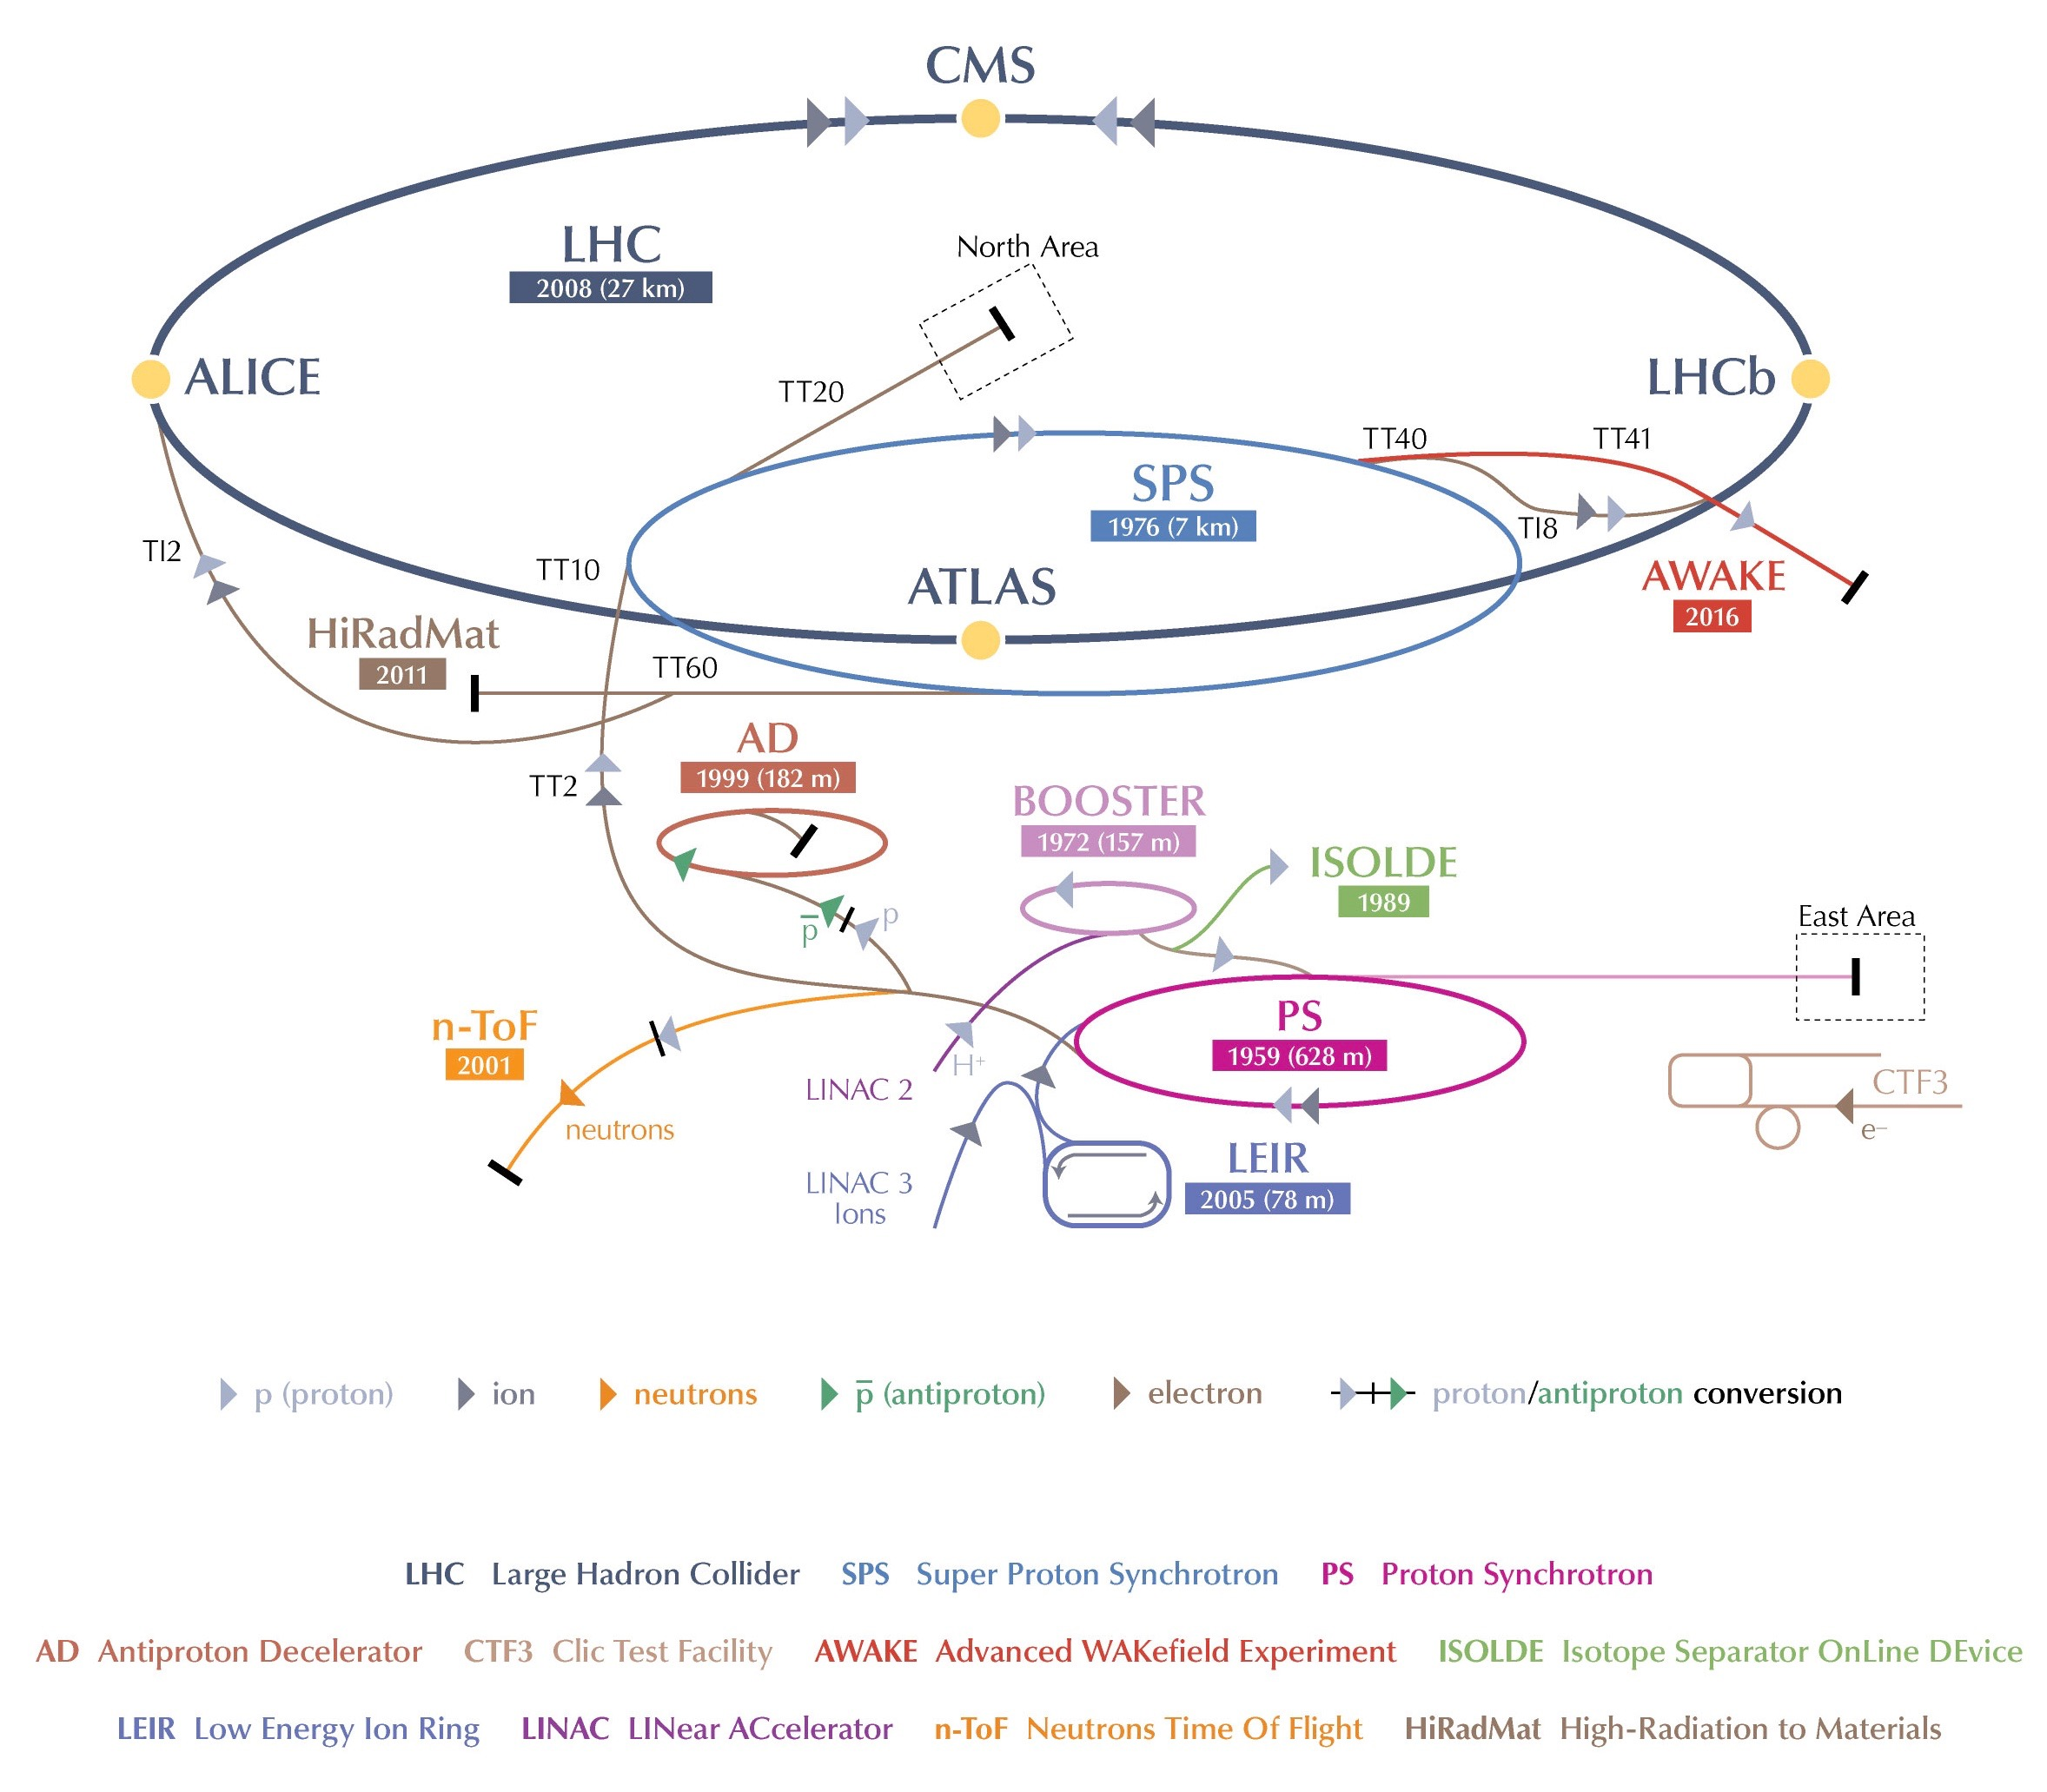
\includegraphics[trim = 125mm 2mm 125mm 90mm, clip, width=0.8\textwidth]{./Figs/LHC_LHCb/accelerator_complex.jpg}
  \caption{The accelerator complex at CERN. The chain of accelerators used to inject protons into the LHC begins with the Linac 2 which accelerates protons to 50~\mev, these are passed to the Proton Synchrotron Booster that accelerates the protons to 1.4 \gev. The Proton Synchrotron is next in the chain, accelerating protons to 25~\gev and creating the desired spacing between proton bunches. Then finally the Super Proton Synchrotron accelerating protons to 450~\gev ready for injection into the LHC. Source: CERN.}
  \label{fig:accelerator_chain}
\end{figure}



The protons leave the chain of accelerators with of energy of 450~\gev per proton and in bunches of \~$10^{11}$ protons, as the bunches are injected into the LHC they are split into two oppositely circulating beams.
The LHC accelerates the protons to the desired centre-of-mass energy using supercooled radio frequency cavities and guides them around the ring with superconducting dipole magnets. %I could add here some details about the magnets and how the LHC accelerates the protons.
Once the required energy has been reached, the bunches are focused using quadrupole magnets before being brought to collided at 4 interaction points around the LHC ring.% at a bunch crossing rate of 40~MHz. 

The centre-of-mass energy of a collider is an important measure of its performance as it dictates what particles could be produced in collisions, another important measure of collider performance is the instantaneous luminosity a collider can provide. The instantaneous luminosity, $\mathcal{L}$, is a measure of how many collision occur per second, it is given by
\begin{equation}
\mathcal{L} = \frac{N^{2} f n_{b}}{\mathcal{F}}.
\label{eq:inst_lumi}
\end{equation}
where $N$ is the number of protons per bunch, $n_{b}$ the number of bunches per beam, $f$ the bunch revolution frequency and $\mathcal{F}$ contains information about the beam geometry. The LHC is designed to operate at a maximum instantaneous luminosity of $10^{34}$~cm$^{-2}$s$^{-1}$. To reach this luminosity the LHC can have up to 2808 proton bunches per beam with a revolution frequency of 11.245 kHz, therefore the separation between proton bunches can be as short as 25~ns. The higher the luminosity, the more collisions happen in a second and the more particles will be produced, this can either be advantageous or disadvantageous depending on the physics process that is being studied.
% and the detector design that records the collisions. 
Therefore luminosity delivered at each interaction point can be tuned by the quadrupole magnets by altering the shape of each bunch to suit the experiments at each point.

Proton beams first circulated the LHC in 2008 and since then there have been two physics runs separated by a long shutdown period. Run 1 began in 2010 and continued until 2013, during this time protons were collided with a centre-of-mass energy of $\sqrt{s}$ = 7~TeV in 2010 and 2011 then this energy was increased to $\sqrt{s}$ =8~TeV for 2012. After Run~1 came first long shutdown (LS1), during this time work was done to prepare the LHC to operate at higher energies and renovation work was preformed on accelerators that provide the LHC with protons. Run~2 began in 2015 with proton collisions at a centre-of-mass energy of $\sqrt{s}$ =  13~TeV, %why 13TeV? I have the answer
this Run will continue until 2018 when a second period of upgrades and maintenance, the Long Shutdown~2, will begin.




There are 7 experiments on the LHC that detect particles produced in proton and heavy ion collisions. There are two general purpose detectors, ATLAS and CMS, that were designed to search for the Higgs boson and new particles that are beyond the scope of the SM in proton collisions, these two experiments operate at the full instantaneous luminosity of the LHC. %Perhaps say we found the Higgs?
ALICE studies quark-gluon plasma produced in heavy ions collisions to understand conditions similar to those present in the early universe. The TOTEM experiment studies properties of protons as they collide head on at the LHC and the MOEDAL experiment is aims to detect magnetic monopoles. The LHCf experiment is a very forward experiment studying particles that are thrown forward in LHC collisions to understand similar processes that occur in cosmic rays. Finally there is the Large Hadron Collider Beauty experiment (LHCb) that will be described in the next section. %, this experiment was designed to studies rare $b$-hadron decays and $\mathcal{CP}$ violating processes and operates at a lower luminosity and has a smaller angular acceptance than the general purpose detectors. %Should probably include the full experiment names as I have done for LHCb or not include the name for LHCb.




\section{LHCb Experiment}
\label{LHCb}

The LHCb experiment was built to study CP violation and rare decays of \bhadrons to search for new physics processes that could be revealed in these decays. At the LHC \bbbar pairs are produced with large transverse momentum, the dominant production mechanisms of \bbbar pairs are gluon-gluon fusion, quark anti-quark annihilation and gluon-gluon splitting. The \bbbar pairs hadronize to form a range of \bhadrons, including $B^{+}$, $B^{0}_{s}$ and $\Lambda^{0}_{b}$, that are studied by LHCb. The large transverse momentum of the \bbbar pairs means that the quarks and subsequent \bhadrons are boosted along the beam pipe. The angular distribution of \bbbar pairs from $pp$ collision is shown in Figure~\ref{fig:bbar_production}. 
\begin{figure}[tb] 
  \centering    
  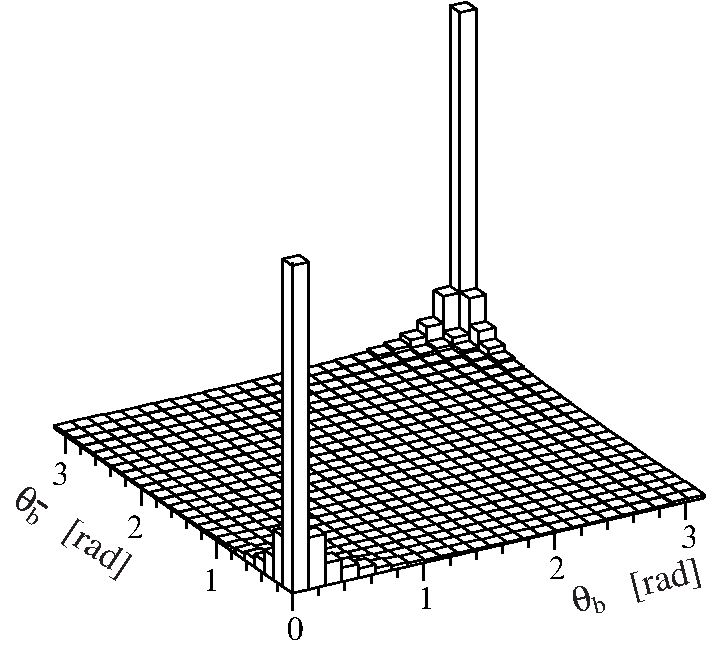
\includegraphics[ width=0.45\textwidth]{./Figs/LHC_LHCb/b_distrib_lhcb.pdf}
  \caption{Simulated angular distribution for \bbbar production at the LHC, angles are relative the the beam pipe with $\theta =0$ in the forward direction and $\theta = \pi$  in the backward direction~\cite{Amato:1998xt}.}
 \label{fig:bbar_production}
\end{figure}



The LHCb experiment was built as a single arm forward spectrometer, with an angular coverage of 10 to 300~mrad in the vertical direction and 10 to 250~mrad in the horizontal direction relative the the beam pipe. This angular coverage what chosen to exploit the small angles relative the the beam pipe that \bbbar pairs are produced at. A cross-section of the detector is shown in Figure \ref{fig:LHCb_detector}, where a right handed coordinate system is used. Protons collide at the interaction point on the left hand side of the diagram, the products of the collisions then travel through the detector leaving information in the different sub detectors along the length of the detector. The information deposited in the sub detectors is reconstructed to determine what happened in the proton collisions. 

\begin{figure}[htb] 
  \centering    
  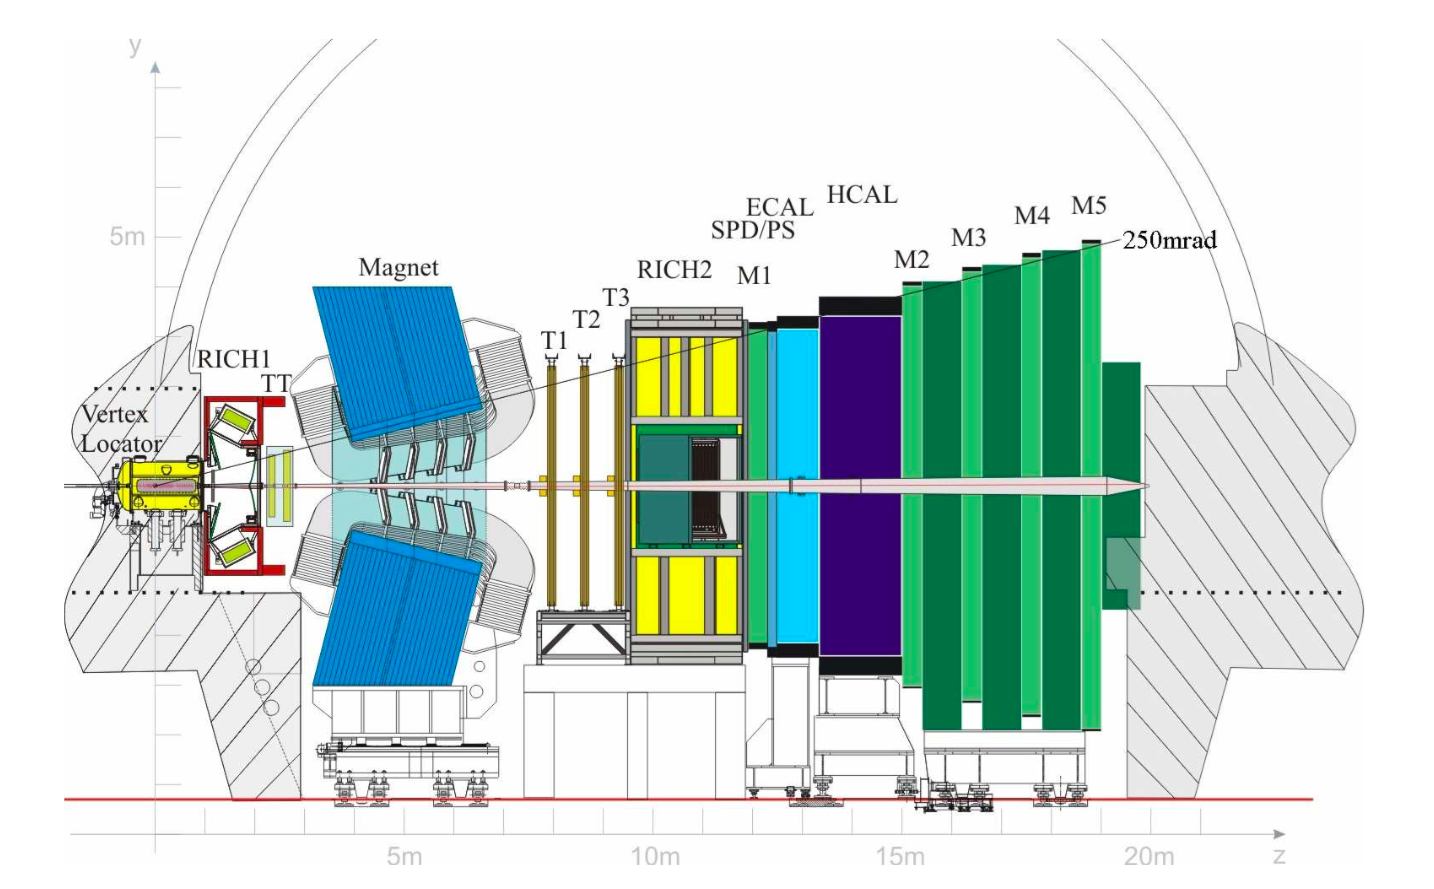
\includegraphics[ width=1.0\textwidth]{./Figs/LHC_LHCb/lhcb.png}
  \caption{Cross section of the LHCb detector \cite{Alves:2008zz}.}
  \label{fig:LHCb_detector}
\end{figure}


The different sub detectors have been chosen to exploit the characteristics of \bhadron decays and fall into 2 distinct categories; tracking detectors and particle identification detectors. These detectors and their performance are described briefly in the following sections along with the trigger system and software needed to preform physics analyses. Finally the data recorded by the experiment during Run 1 and Run 2 is presented in Section \ref{LHCb_data}. For a full description of the detector and its performance during Run 1 see references \cite{LHCb:2003ab,Aaij:2014jba}.




\subsection{Tracking}
\label{Tracking}

The tracking system within the LHCb experiment consists of the VELO, the dipole magnet and the tracking stations, together the sub-detectors provide precise information on the passage of charged particles through the detector and the particle momentum. 
The tracking detectors work on the basic principle that the passage of high energy charged particles through silicon or ionised gas causes excitation or ionisation atoms in the material. The release of this energy is recorded and translated into an electrical signal that reveals the path of a particle. 
Precise particle track and momentum measurements are necessary to obtain the accurate particle mass and decay time measurements that help distinguish between different \bhadron decaying in the LHCb detector. 

\subsubsection{The VELO}
\label{VELO}
The VELO is a silicon detector surrounding the interaction point. Its main goal is to provide precise information about the interaction vertices and secondary decay vertices of particles produced in proton collisions. Information the VELO provide enables precise measurements of particle lifetimes and impact parameters of particles tracks necessary for physics analyses.


The VELO is made up of two identical halves, each half consists of 21 stations containing two silicon sensors arranged along the beam pipe. The two halves of the VELO slot together and there is a small hole in the centre of the sensors for the beams to pass through. The arrangement of sensors along the $z$ axis, shown in figure \ref{fig:velo}, it designed such that the sensors cover the full LHCb acceptance and a charged particle within the acceptance will pass through at least three stations. In each station the two sensors measure different coordinates, one measures the $r$ coordinates of charged particles and the other measures the $\phi$ coordinates as shown in Figure~\ref{fig:velo_sensor}. The $r$, $\phi$ coordinates and the $z$ placement of the sensors are used to reconstruct charged particle trajectories. Cylindrical coordinates were chosen to allow for fast reconstruction for particle trajectories in the VELO.

\begin{figure}[htb] 
  \centering    
  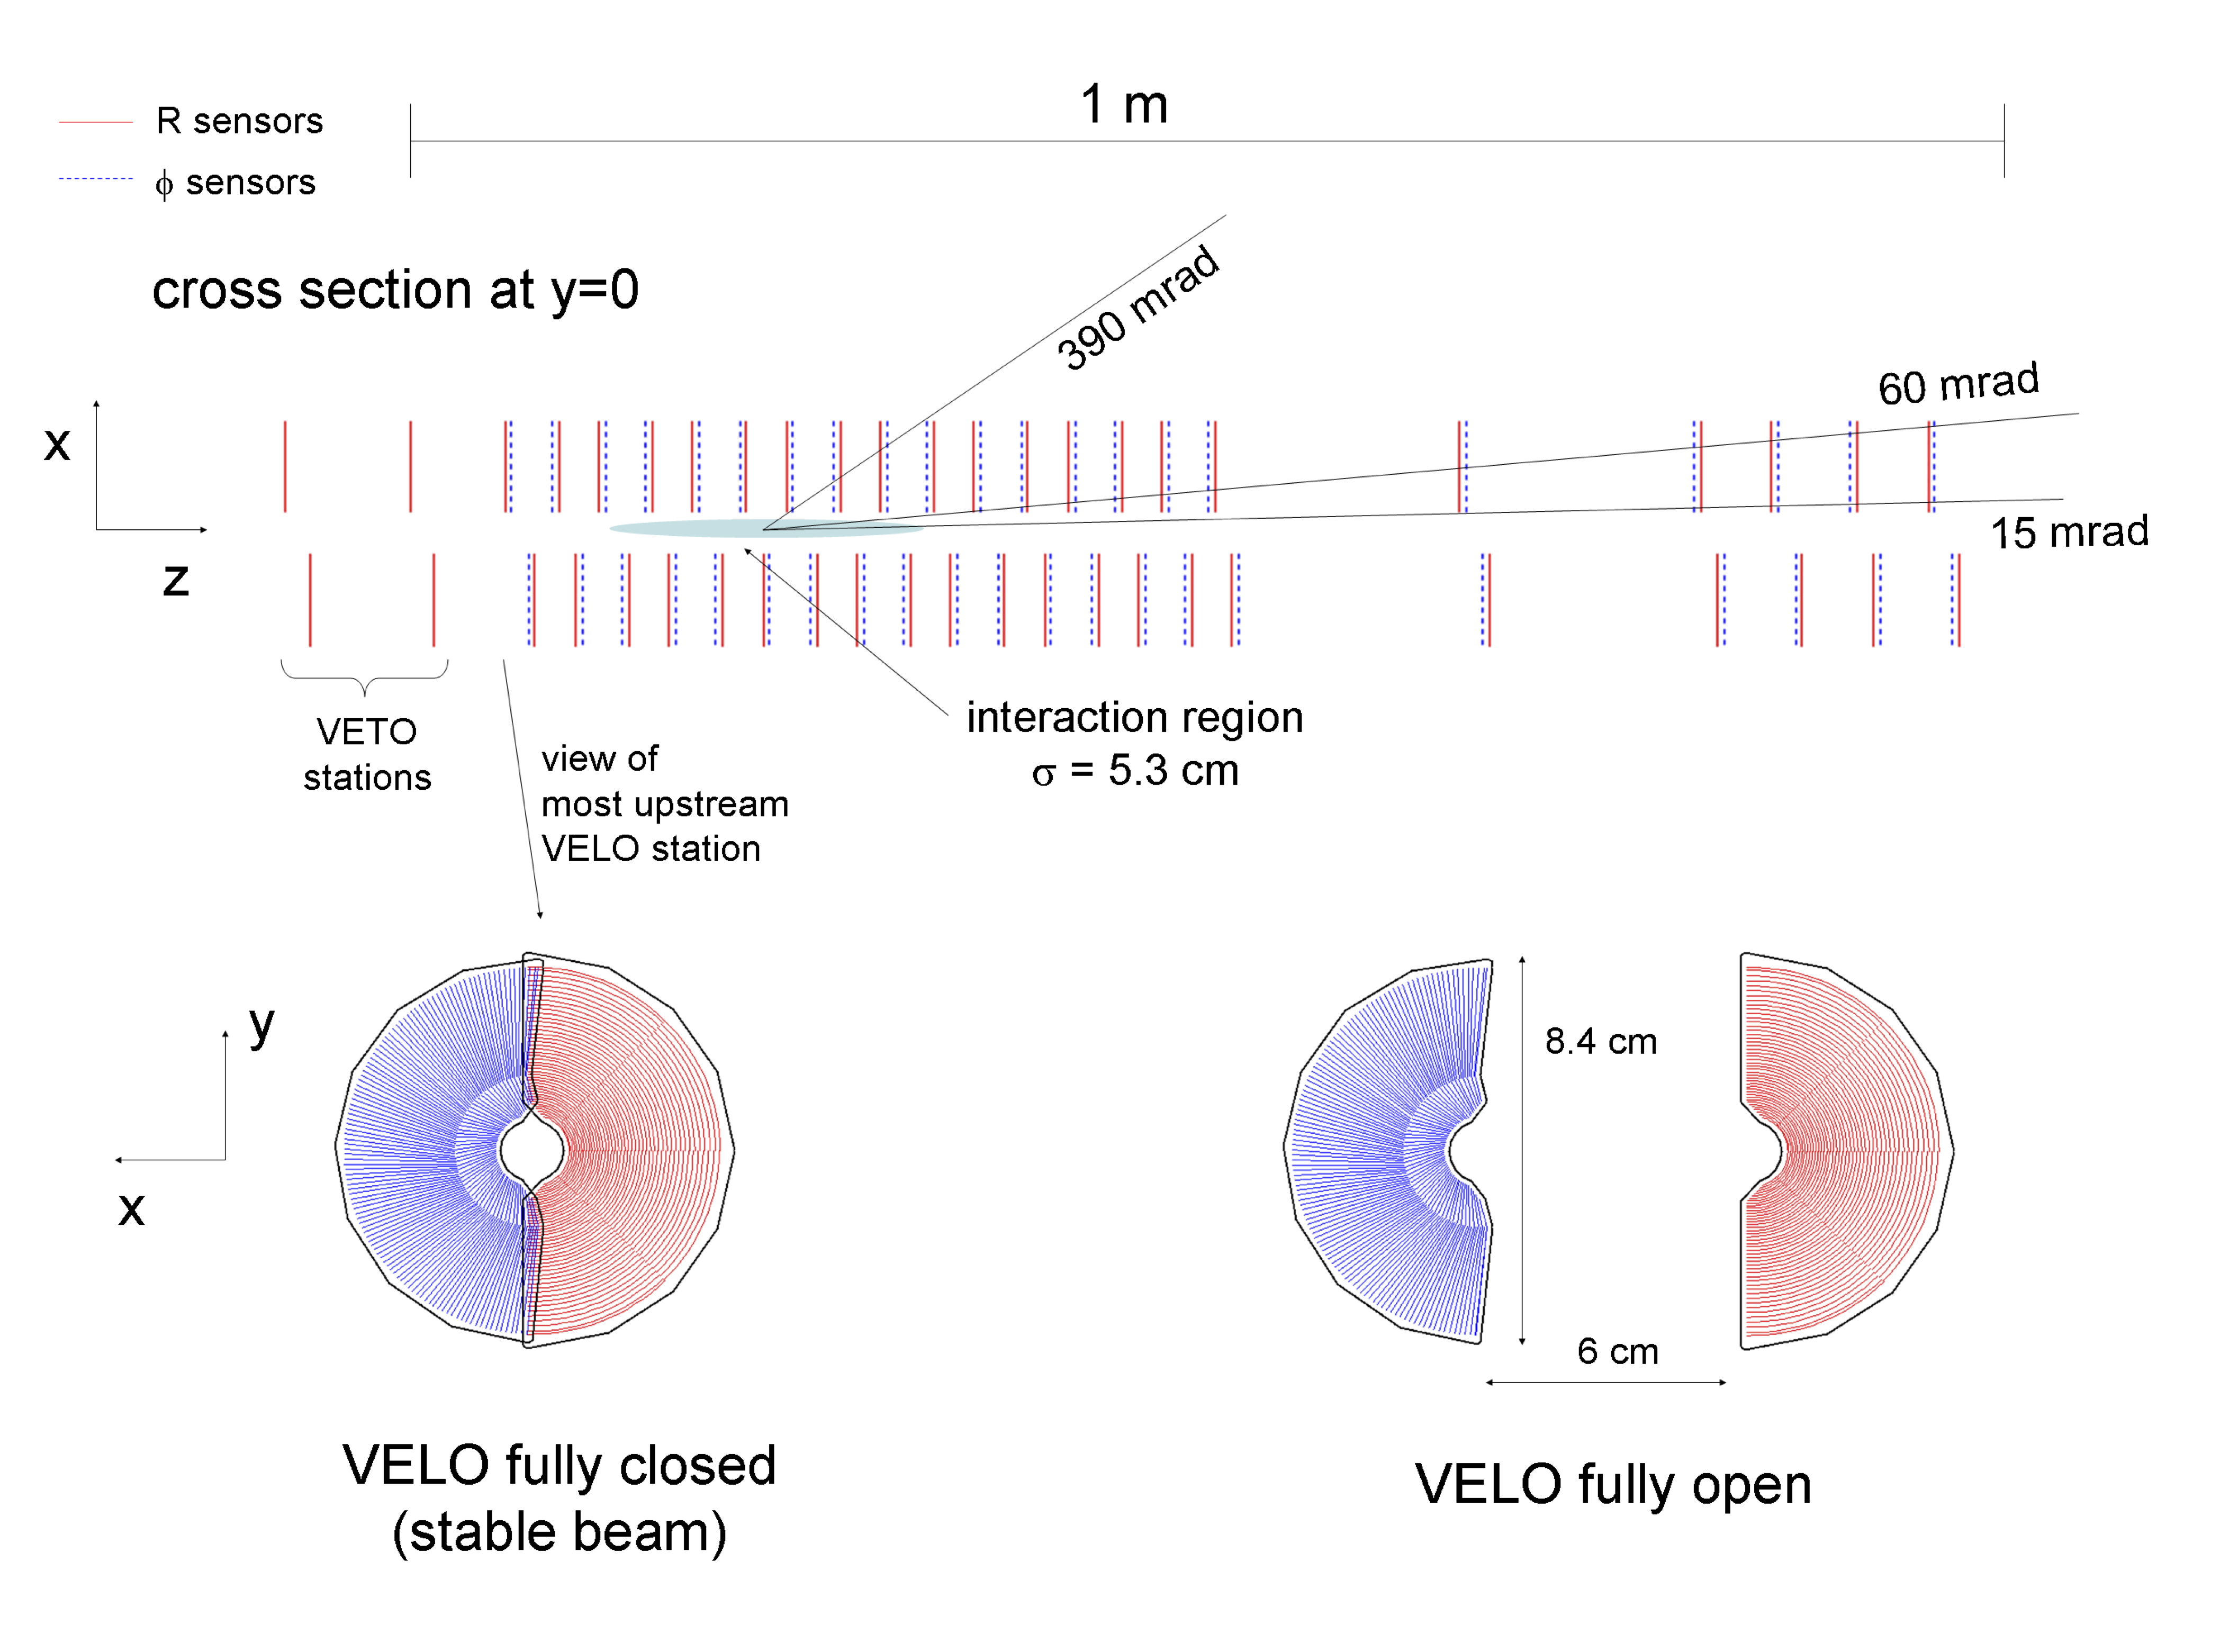
\includegraphics[ width=0.7\textwidth]{./Figs/LHC_LHCb/velo.png}
  \caption{The VELO layout and position of sensors along the beam axis \cite{Alves:2008zz}.}
  \label{fig:velo}
\end{figure}


\begin{figure}[htb]
  \centering
  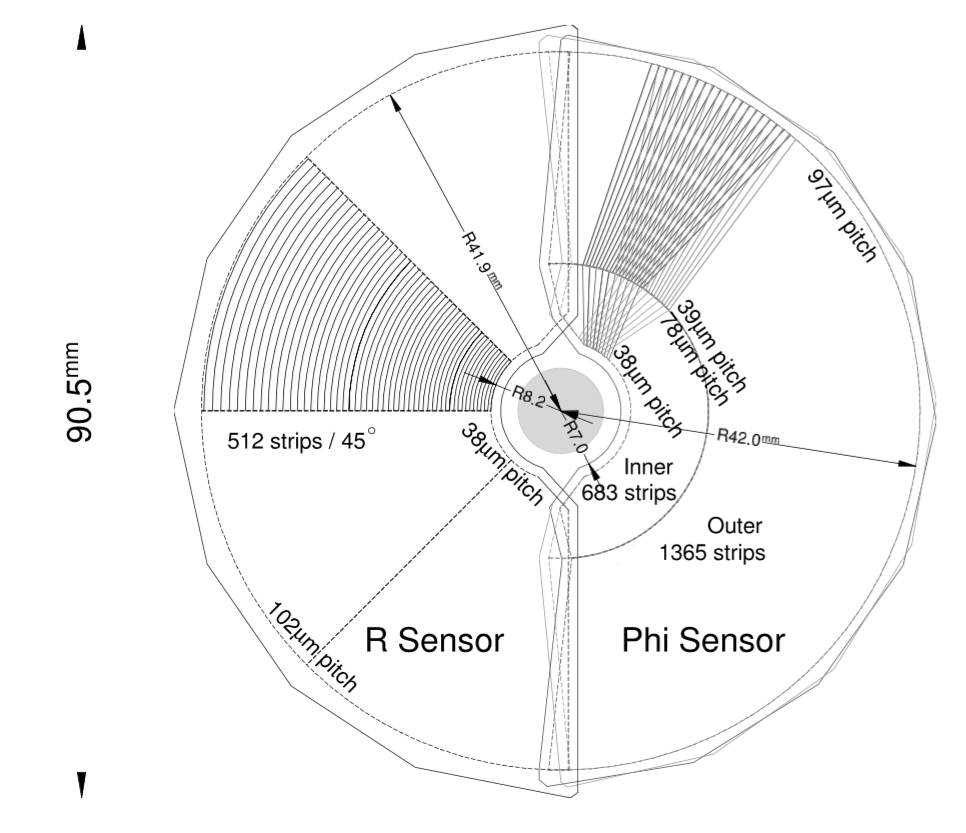
\includegraphics[ width=0.6\textwidth]{./Figs/LHC_LHCb/Velo_sensor_diagram.png}
  \caption{Diagram of $r$ and $\phi$ sensor layouts~\cite{Alves:2008zz}.}
  \label{fig:velo_sensor}
\end{figure}


The momentum resolution achievable for charged tracks is limited by multiple scattering of particles as they travel through material in the detector. Therefore, to ensure good momentum resolution throughout the detector, the VELO is kept in a vacuum to reduce its material budget. Each half of the VELO is enclosed inside an aluminium box, which keeps it in a vacuum and shields the electronic readouts of the from radio frequencies generated by the beam. The overall material budget of the VELO comes to 17.5 $\%$ of a radiation length.

Excellent vertex resolution is required in the VELO, to achieve this the sensors in the VELO need to be as close as possible to the interaction point. This is achieved by making the VELO out of two retractable halves and including the interaction point within the coverage of the VELO. During data taking, when the VELO is recording particle tracks the sensors are only 8mm from the beam axis. However during the injection phase of the beam the width of the beam is much greater, therefore the 2 halves of the VELO can retract so that they are 3~cm from the nominal beam axis. This keeps the VELO safe from unnecessary radiation damage. The two halves of the VELO are displaced by 150~mm in the $z$ direction, as shown in Figure~\ref{fig:velo} so that when the VELO is closed, the sensors in each half overlap to help with detector alignment and reduced edge effects. 

%\begin{figure}[htb] 
%  \centering    
%  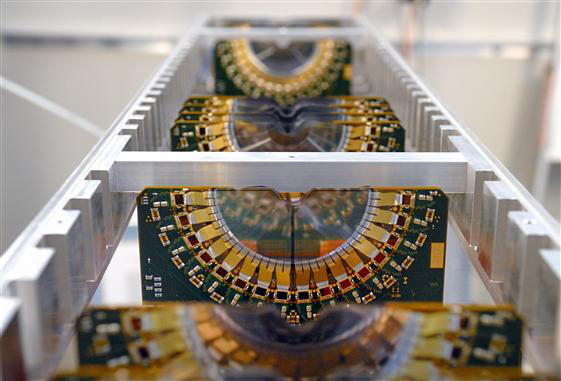
\includegraphics[ width=0.7\textwidth]{./Figs/LHC_LHCb/Velo_photo.jpg}% ./Figs/Detector/Velo_photo.jpg}
%  \caption{The velo Soure: LHCb.}
%  \label{fig:velo_photo}
%\end{figure}


An additional purpose of the VELO is to act as a veto for high pile up events. There are 2 VELO sensors upstream of the interaction point that provide information to the trigger about how many $pp$ interactions there were with each bunch crossing. Events with large numbers of primary vertices are difficult and time consuming to reconstruct and lead to less precise measurements of particle decay properties. Information from the VELO is used to reject events with high numbers of primary vertices to ensure the best used of information from the detector.

The VELO achieves a vertex resolution of 10 - 20~$\mu$m transverse to the $z$ direction and 50 - 100 ~$\mu$m along the $z$ direction, the resolution of each track depends on the number of tracks in each event as shown in Figure~\ref{fig:Velo_PV_resolution}. The VELO also gives measurements on the impact parameters of particles tracks, which is the distance of closest approach between a particle track and the primary vertex. Figure \ref{fig:IP_res} shows the IP resolution for 2012 data, for a track with transverse momentum of 1~GeV/c is has an impact parameter resolution of 35~$\mu$m. 



%Can I just put the track resolution possible with the VELO?
\begin{figure}[tb] 
  \centering    
  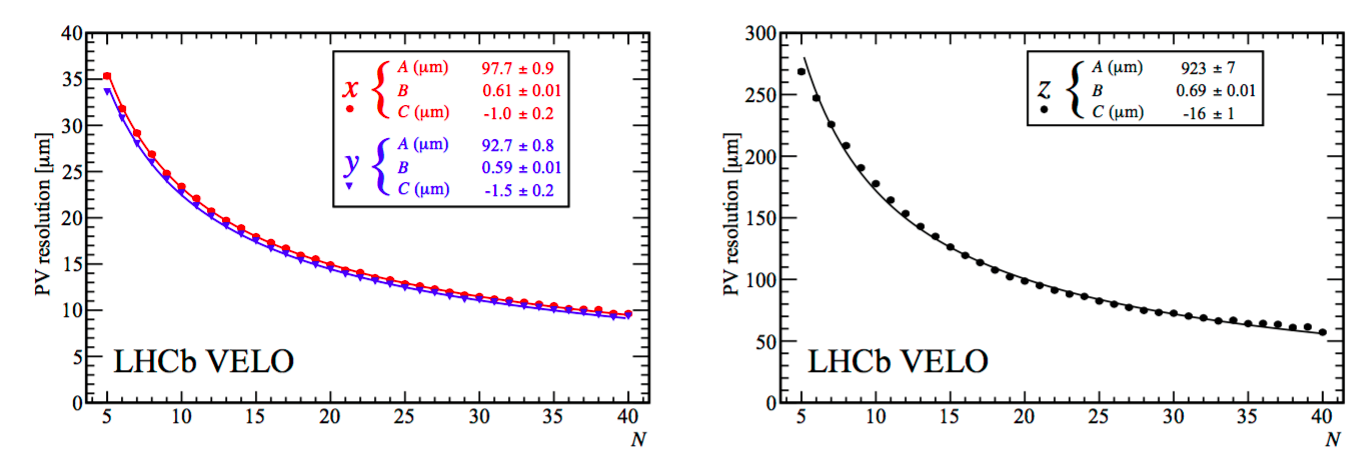
\includegraphics[ width=1.0 \textwidth]{./Figs/LHC_LHCb/Velo_vertex_resolution.png}
  \caption{Velo performance for primary vertex resolution perpendicular (left) and parallel (right) to the beam axis as a function of the number of tracks in an event for 2012 data~\cite{LHCbVELOGroup:2014uea}.}
  \label{fig:Velo_PV_resolution}
\end{figure}


\begin{figure}[tb] 
  \centering    
  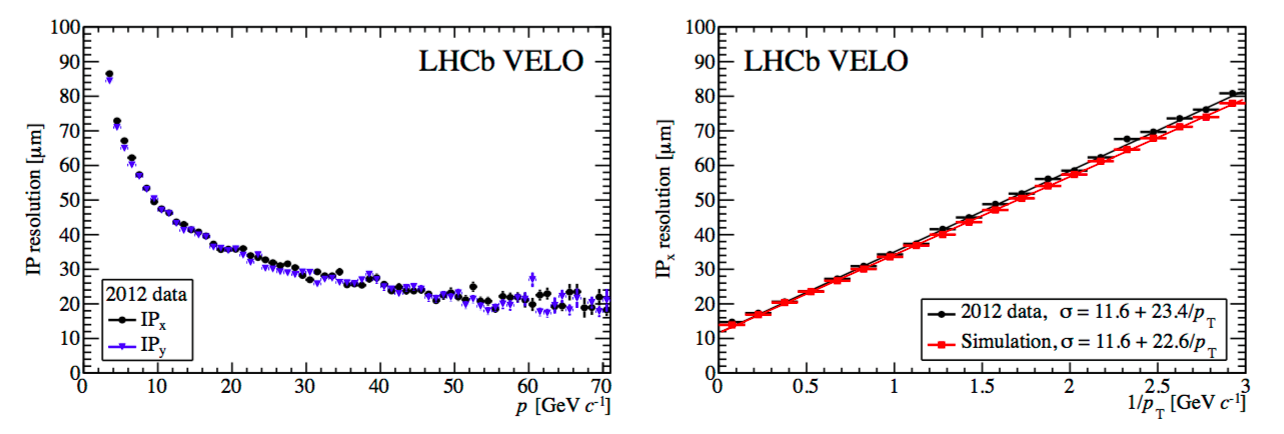
\includegraphics[ width=1.0\textwidth]{./Figs/LHC_LHCb/Velo_IP_resolution.png}
  \caption{Velo performance for impact parameter resolution as a function of momentum (left) and inverse transverse momentum (right) for 2012 data~\cite{LHCbVELOGroup:2014uea}.}
  \label{fig:IP_res}
\end{figure}


%Overall the VELO gives such and such precision.  vertex resolution in the transverse plane 10-20 mircons, in the z directions 50-100 microns depending on the number of tracks in the vertex. %The VELO is also important the impact parameter resolution and decay time resolutions.  (This may go at the end so that everything for tracking is together?) best resolution is 4 micrometers which allows a lifetime measurement of 50 fs. (Performance paper)



\subsubsection{The Tracking Stations} 
\label{Tracking_Stations}
The LHCb experiment has 4 tracking stations in addition to the VELO, the Tracker Turicensis (TT) which is located upstream of the magnet and the T stations, T1-T3, located down stream of the magnet. These tracking stations provide complementary tracking information to the VELO and the presence of the magnetic field allows the momentum of charged particles to be determined. 



The TT is made up of 4 layers of silicon trackers spaced 27 cm apart that cover the full LHCb angular acceptance. The TT is located just within the influence of the magnetic field of the dipole magnet, which provides the detector with 2 main purposes. Firstly, the TT tracks the passage of charged particles with high momentum to enable good momentum resolution for tracks when combined with the other tracking stations. The TT has a resolution of 50~$\mu$m for a single hit, this resolution was chosen so that multiple scattering in the detector material rather than detector resolution is the limiting factor for the momentum resolution. The second purpose of the TT is to record tracks of low momentum particles that are then swept out of the detector acceptance as they continue through the magnetic field. These tracks will have a lower momentum resolution but help with pattern recognition within the RICH detectors. 
%Information from just the TT and the VELO can provide an momentum accuracy of ~ 20 $\%$. 
%active area of 8.4m^2


The T stations, T1-3, are split into two sections, each are composed of an Inner Tracker (IT) made of silicon and an Outer Tracker (OT) composed of straw drift tubes. 
There is a large increase in size of the tracking stations between the TT and the T3 so that all the detectors cover the full angular acceptance of the detector.  The TT is 150 cm by 130 cm where as the T3 station is 600cm by 490 cm, this is illustrated in Figure \ref{fig:size_of_tracking_stations}. The large size of the T stations meant that the high cost of silicon prevented it being used for the full coverage of each station.

\begin{figure}[htb] 
  \centering    
  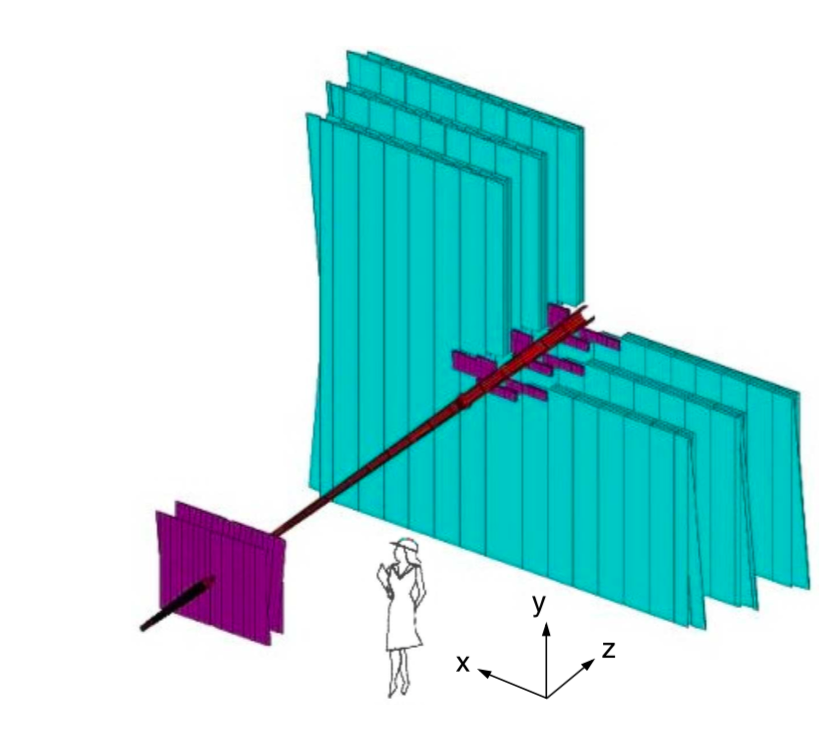
\includegraphics[ width=0.5\textwidth]{./Figs/LHC_LHCb/TT_IT_OT_comparison.png}
  \caption{Sizes of the TT and T stations~\cite{Alves:2008zz}.}
  \label{fig:size_of_tracking_stations}
\end{figure}

The IT has very similar in design to the TT, each station is made of 4 layers of silicon trackers and it has with a track resolution of 50 $\mu$m.
%and has an active area of 4.0m2. 
The silicon trackers are arranged in a cross shape around the beam pipe, as shown in Figure \ref{fig:size_of_tracking_stations}, although the IT covers less than 2$\%$ of the T stations, 20$\%$ of tracks pass through it. This allows the occupancy of the OT to be less than 10$\%$ enabling a good overall track resolution from the OT despite it not being made of silicon. The OT of each tracking station is made of 2 staggered layers of straw tubes, they cover the remaining area required for cover the LHCb full angular acceptance which includes tracks bend by the magnetic field. The tubes have a fast drift time of 50~ns giving a better than 200~$\mu$m track resolution. 


\subsubsection{The Dipole Magnet}
\label{Magnet}
A warm dipole magnet is used to measure the momentum of charged particles travelling through the LHCb detector. In a magnetic field the trajectories of charged particles are bent and from the radius of curvature of the particle track the particle momentum can be determined.

The magnet is located between the TT and the T stations and its field covers the full LHCb acceptance. The field is in the vertical direction therefore bending tracks in the horizontal direction. The magnet was designed so that the field strength in the RICH detectors is negligible (less than 2 mT) and to have the largest strength possible between the TT and T stations. Figure \ref{fig:Magnet_field} shows a plot of the magnet strength alongside the detector layout. A small magnetic field is achieved in the RICH detectors by iron shielding. The magnet was designed to have an integrated field strength is 4Tm for track that travels 10m through the detector.% and the peak strength is 1.1T. % I should maybe mention the measurement of the field and how it had to be accurate (with Hall probes) in order to get good momentum resolution but I don’t want to. The magnetic field strength enables the tracking systems to achieve a momentum resolution of $\delta p / p \~0.4\%$. 

\begin{figure}[htb]
  \centering
  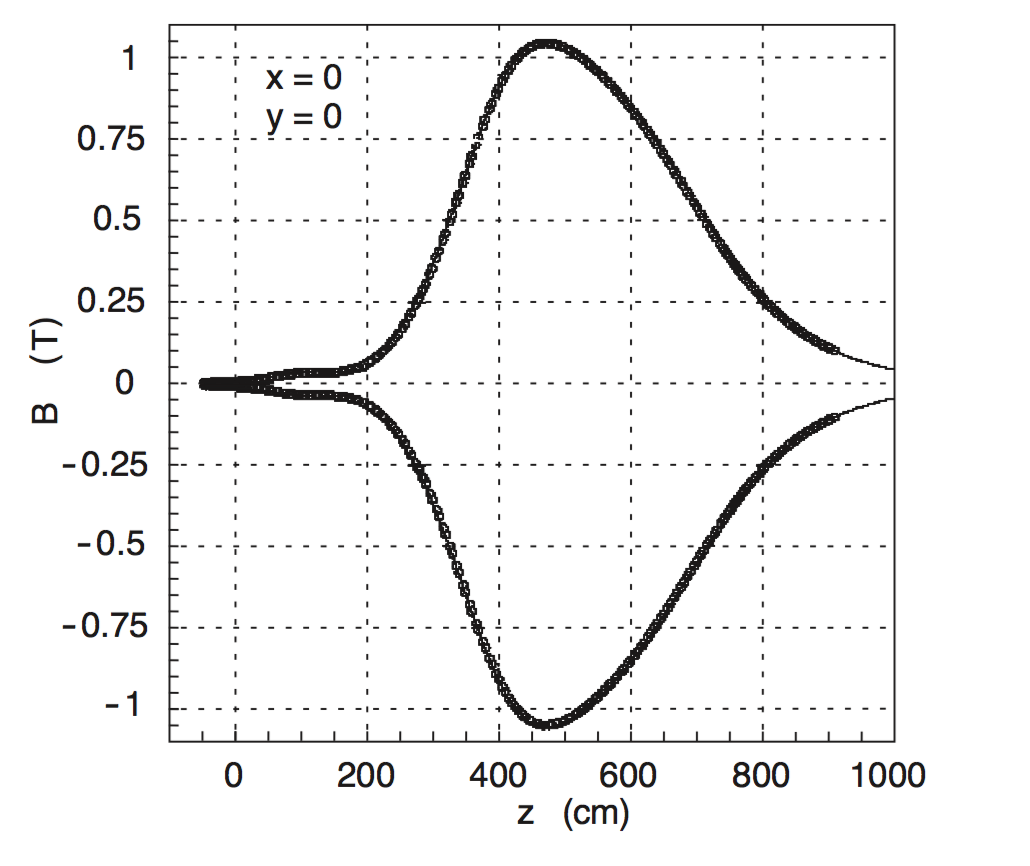
\includegraphics[ width=0.4\textwidth]{./Figs/LHC_LHCb/Magnet_field.png}
  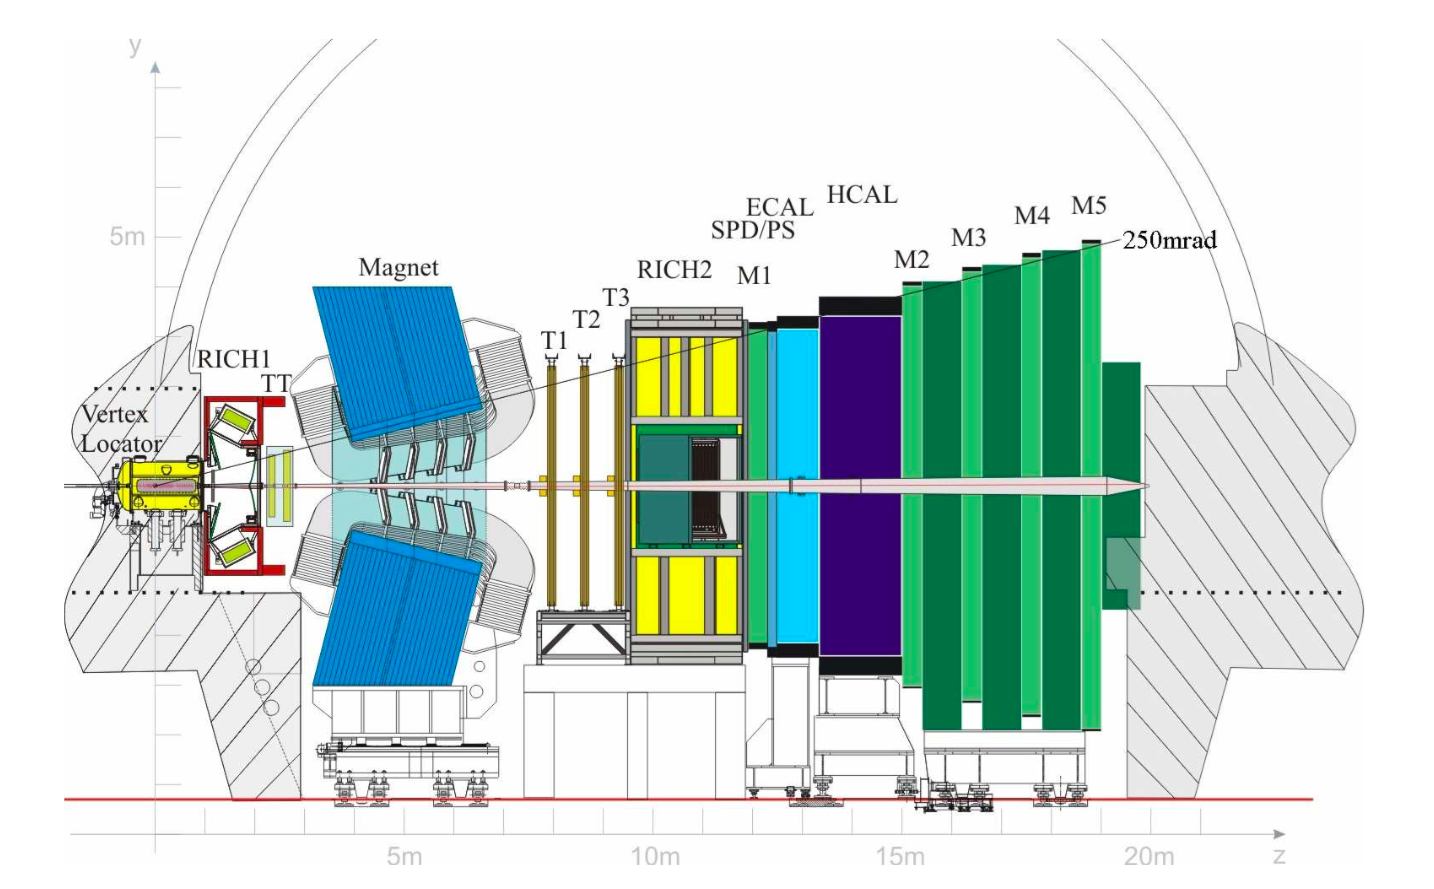
\includegraphics[ width=0.48\textwidth]{./Figs/LHC_LHCb/lhcb.png}
  \caption{Magnet field of the dipole magnet along the length of the LHCb detector (left) and the layout to the LHCb detector \cite{Alves:2008zz}. The peak strength of the field occurs between the TT and T1-3 station. }
  \label{fig:Magnet_field}
\end{figure}

%\begin{figure}[tb] 
%  \centering    
%  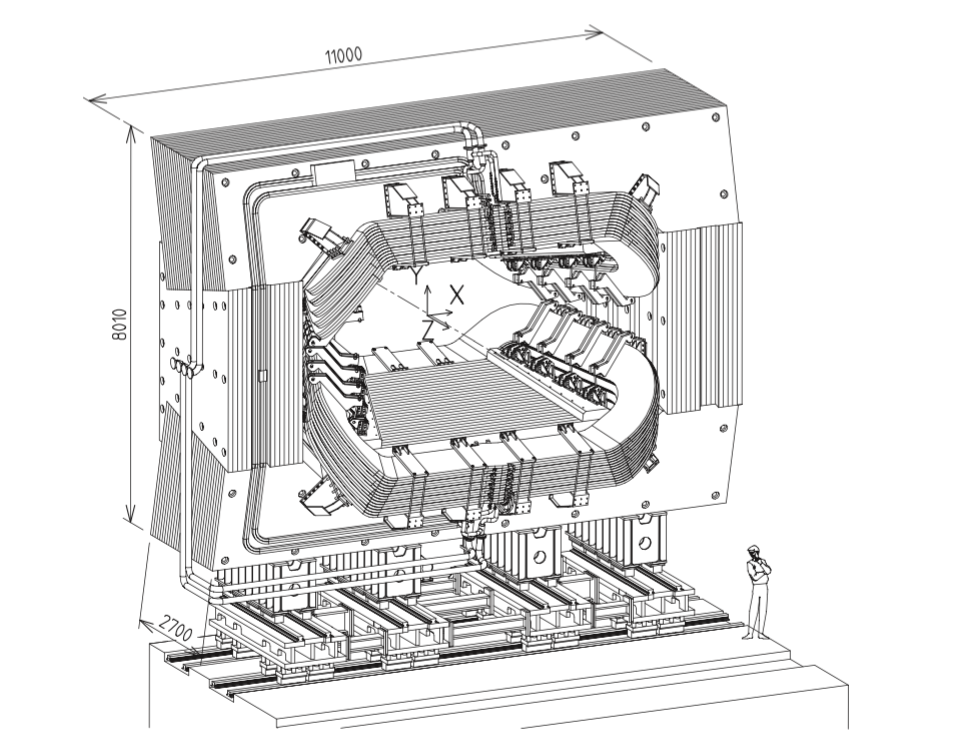
\includegraphics[ width=1.0\textwidth]{./Figs/LHC_LHCb/Magnet_picture.png}
%  \caption{Magnet picture. Source: \cite{Alves:2008zz}.}
%  \label{fig:types_of_tracks}
%\end{figure}


The polarity of the magnetic field is periodically switched so that is bends charged tracks in opposite directions. This is done so measure left-right detection asymmetries and to help understand systematic uncertainties of CP violation measurements. % These are not relevant for B2mm.



\subsubsection{Track reconstruction and performance}
\label{Track_recon}


The information left by the passage of charged particles in the VELO, TT and T stations is combined using track reconstruction algorithms to find trajectories of charged particles though the length of the LHCb detector and the particle momentum.  
The algorithms start with either segments of tracks in the VELO or the T stations as seeds and extrapolate from these segments into the other tracking detectors in specific search windows. 
Once the segments of the track have been found the trajectory is fitted with a Kalam Fitter with takes into account multiple scattering and energy loss within the detector. For each track the fitter returns the $\chi^{2}$ per degree of freedom, this is a measure of quality for the track. In LHCb this parameter is used to ensure that only good quality tracks are used in physics analyses. 
The reconstructed tracks are classified into five types depending on which detectors they travelled through, as shown in Figure \ref{fig:types_of_tracks}.



The different track classifications are:
\begin{itemize}
\item {\bf VELO tracks} are formed by particles produced at large angles to the beam axis or travelling in the negative $z$ direction from the interaction point, these particles only leave tracks in the VELO. These tracks are useful for reconstructing primary vertices.  
\item {\bf Upstream tracks} are made by low momentum particles that only leave hits in the tracking stations upstream of the magnet, the VELO and TT. The absence of tracks further down the detector is because the magnetic field sweeps the particles out of the detector acceptance. Upstream tracks have poor momentum resolution but are useful for understanding backgrounds and pattern recognition in the RICH~1 located between the VELO and the TT.
\item {\bf Downstream tracks} are produced by decays of long lived neutral particles, that travel out of the VELO before decaying. These particles only leave tracks the TT and T stations. 
\item {\bf T tracks} are tracks that only cross the T1-3 stations and are formed from particles created in interactions with the detector material. Similarly to upstream tracks, T tracks can help to understand backgrounds and pattern recognition in the RICH~2 located just before the T stations.
\item {\bf Long tracks} are the most useful for physics analyses because they are formed by particles that travel through the VELO, TT and T1-3 stations. Information from all the tracking stations is combined so these tracks have the best momentum resolution.
\end{itemize}


\begin{figure}[tb] 
  \centering    
  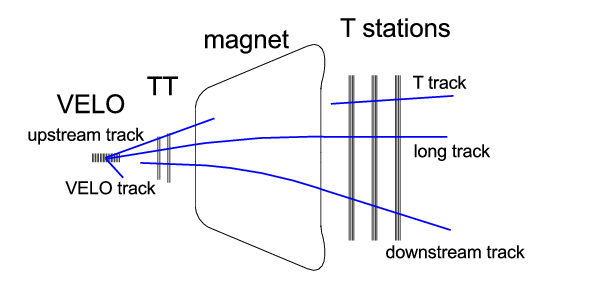
\includegraphics[ width=0.8\textwidth]{./Figs/LHC_LHCb/Types_of_tracks.png}
  \caption{Different types of tracks that are reconstructed at LHCb~\cite{Aaij:2014pwa}.}
  \label{fig:types_of_tracks}
\end{figure}

The efficiency to correctly reconstruct tracks varies with different parameters of the events, including the momentum to the particle producing the track and the number of tracks present in the event, as shown in Figure~\ref{fig:types_of_tracks} for 2012 data. In Run 1 long tracks were correctly reconstructed on average of 96$\%$ of the time.





\begin{figure}[tb] 
  \centering    
  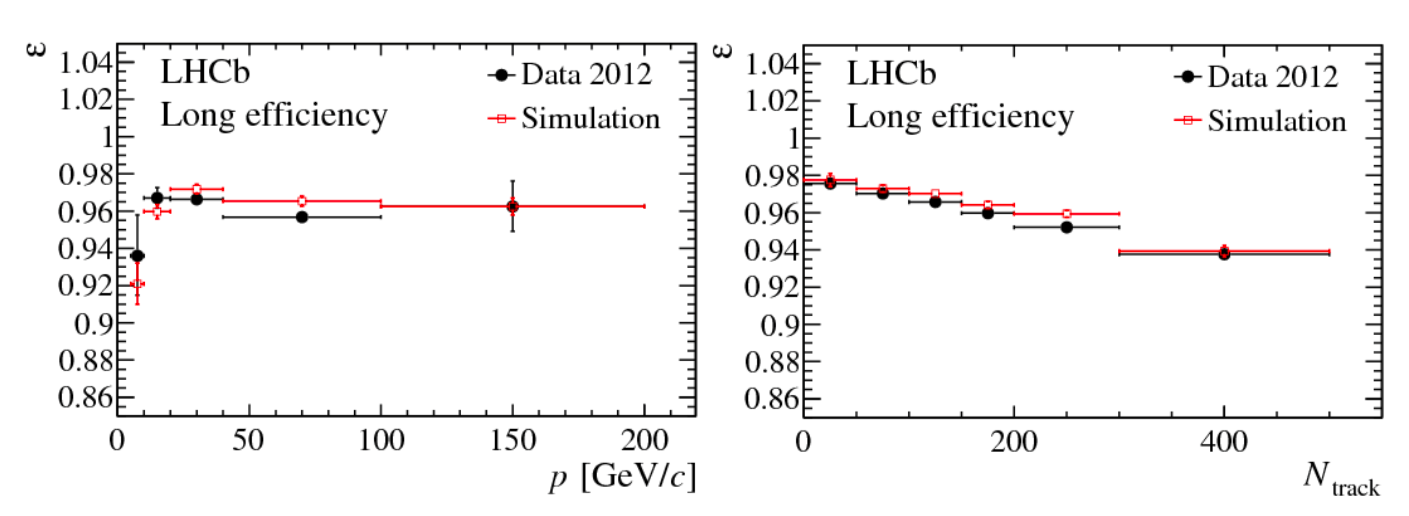
\includegraphics[width=1.0\textwidth]{./Figs/LHC_LHCb/LongTrack_efficiencies.png}
  \caption{Long track reconstruction efficiency as a function of momentum (left) and number of track in the event (right) for 2012 data \cite{Aaij:2014pwa}.}
  \label{fig:types_of_tracks}
\end{figure}




Inevitably not all tracks that are reconstructed are correct, there are two main types of incorrectly reconstructed tracks. The first are clone tracks that occur when the two tracks have many hits in common, when this happens the track with the highest number of total hits it used and the other is discarded. The second type of incorrect tracks are ghost tracks when track segments in different detectors are incorrectly joined together. This most offen occurs with segments in the VELO and T1-3 stations, the number of ghost tracks in an event depends on the event multiplicity. These tracks are removed by cutting on the output of a neural network that returns a probability of how likely a track is to be fake.



Once the tracks have been reconstructed, parameters that are necessary for the identifying and measuring different particles decays in an event can be computed from the tracks. The combined tracking systems achieve a momentum resolution of $\delta p / = 0.5\%$ for particles with $p$ =  20~GeV/c and a resolution of $\delta p / = 0.8\%$ for particles with $p$ =  100~GeV/c.  This momentum resolution, when combined with vertex information from the VELO, gives a decay time resolution of around 50~ns. 



%The performance of the tracking system has been studied of Run 1 data \ref{ performance paperS}. The tracking system provide measurement of the momentum of the charged particles that it tracks, good momentum resolution is required in order to obtain good mass resolution which is necessary to identify different  b hadrons and to distinguish between signal and background events. The momentum resolution of long tracks is shown in figure  OR the momentum resolution is $\delta$p/p = X - Y $\%$ which depends on the momentum of the reconstructed track. 


%The tracking system allows accurate reconstruction of primary vertices, this is necessary to measure time dependant processes, lifetimes and identify decaying particles. It was particular important for LHCb so that is could measure the rapidly oscillation Bs system. The PV resolution has been measured on 2012 data and varies with the number of tracks used to reconstruct the vertex, on average the vertex resolution transverse to the beam is between 10 and 25 mum and parallel to the beam is  between 50 and 150 mum for the z direction as shown in figure \ref{fig:types_of_tracks} for 2011 data. %Ref veto paper.



%The impact parameter is another important variable, it measure the distance of closest approach of a track to the PV, long lived particles tend to have a large IP wrt to PV because they travel before they decay. Good measurements of the IP help to remove prompt backgrounds. The IP resolution depends on the momentum of the particles and Figure \ref{fig:types_of_tracks} shows the IP resolution for 2012 data, for a track with transverse momentum of 1 GeV/c is has an IP resolution of 35 mum.

%Finally, the measurement of lifetime of b hadrons at LHCb needs accurate decay time measurements but more importantly to understand the rapidly oscillating Bs system good decay time resolution is needed. To reconstruct the decay time information about particle momentum and decay length, how far the particle travelled before it decays are needed. Therefore good PV resolution and moment resolution are needed. The LHCb detector achieved typically 50 ns resolution on the decay time. 



\subsection{Particle Identification}
\label{PID}

In LHCb the particles identification (PID) detectors consist of two ring imaging Cherenkov (RICH) detectors, electromagnetic and hadroics calorimeters and the muons stations. Together these detectors distinguish between different charged leptons and hadrons and between neutral particles such as photons and neutral pions. Good particle identification is necessary to determine which \bhadron decayed and to distinguish between topologically similar decays, such as \bdkpi, \bskk and \bmumu. %This could be out elsewhere perhaps in the RICH specific part?



\subsubsection{RICH}
\label{RICH}
%There is a plot that shows the usefulness in comparing 2 mass plots of the RICH PID, this is in Ed Greening's Thesis. It could be nice to include this, or something like it because it is very relevant to Bs2MuMu and the verification of the lifetime measurement methods that I did. 

RICH detectors are used at LHCb to distinguish between charged hadrons and leptons that have a momentum between 0 and 100~GeV/c. The RICH detectors are vital to distinguish between pions, kaons and protons frequently produced in \bhadron decays. %This needs to be done because correctly reconstructing the b hadron invariant mass relies on correctly identifying what it decayed into. Information from the RICH is particularly important at distinguishing different b2hh decays which is useful for this thesis. 
The energy range of the RICH detectors was chosen because the typical decay products of 2-body \bhadron decays is around 50~GeV. 



The RICH detectors are based on the following principle; when a charged particle travels with velocity $v$ through a dielectric medium with a refractive index $n$, the atoms excited by its passage are polarised, if the particle is travelling faster than the speed of light in the medium the excitation energy is released as a coherent wavefront. The angle, $\theta_{c}$, the wavefront travels at relative to the particle trajectory depends on the speed at which the particle was travelling as $cos(\theta_{c}) = c/nv$. The light produced is called Cherenkov radiation. The RICH detectors measure the angle of light produced as particles pass through them, the angle gives a measurement of the particle’s speed which when combined with momentum from the tracking stations gives that particle’s mass and therefore its identity. 


\begin{figure}[htb]
  \centering
  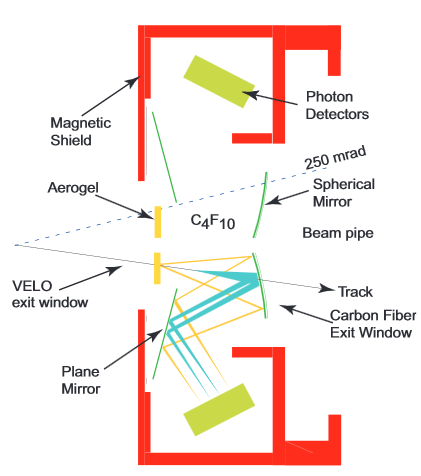
\includegraphics[ width=0.40\textwidth]{./Figs/LHC_LHCb/RICH1diagram.png}
  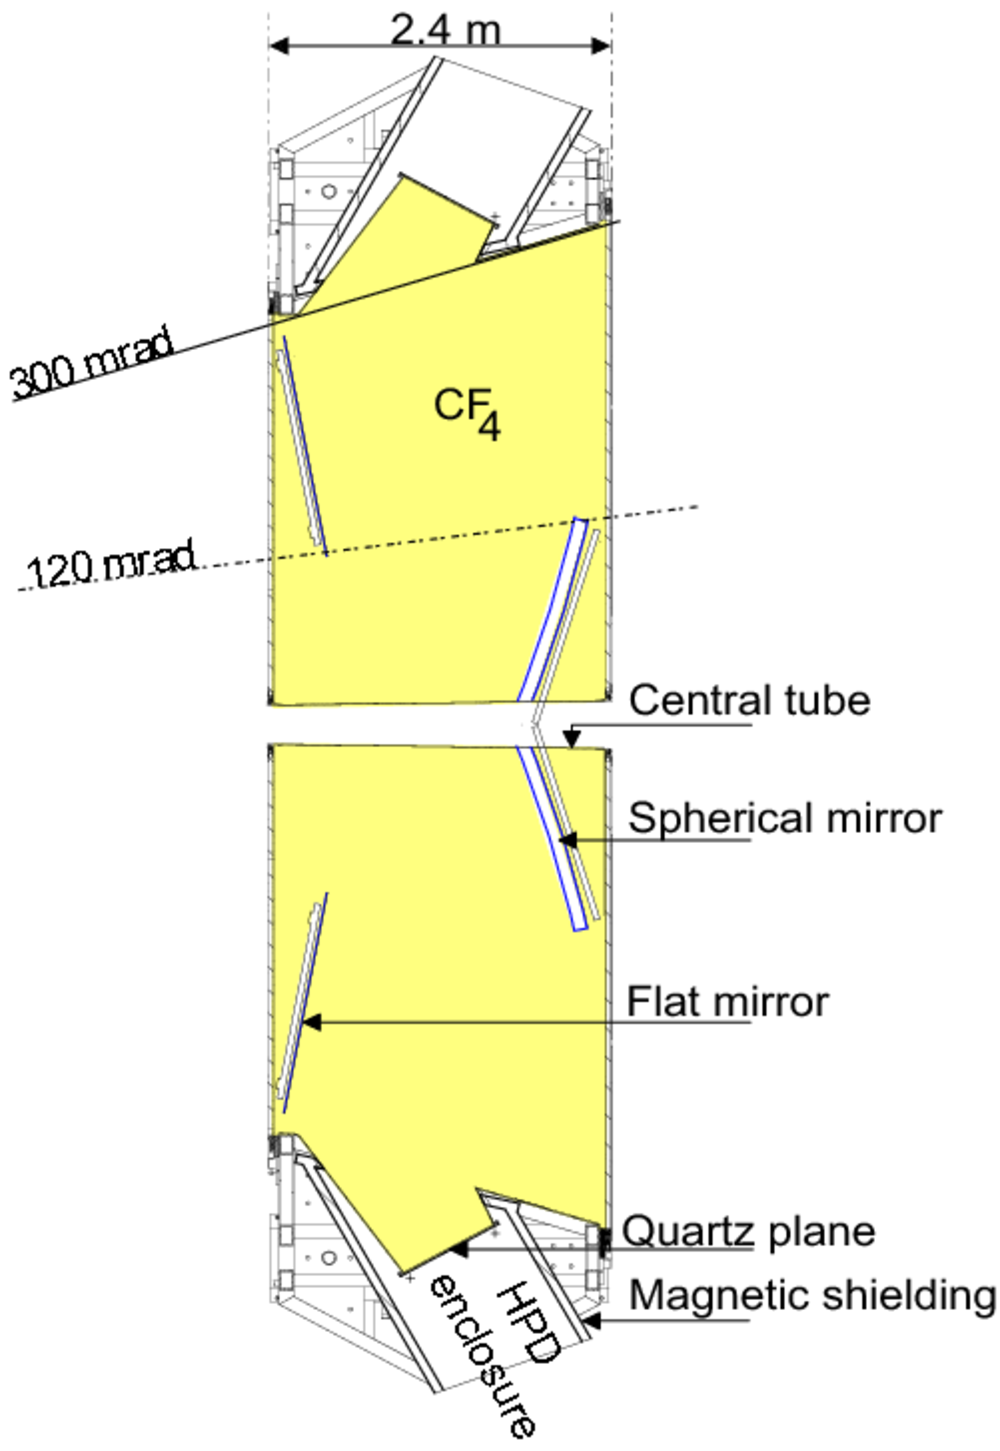
\includegraphics[ width=0.3\textwidth]{./Figs/LHC_LHCb/rich2_schematic.png}
  \caption{Diagram of the RICH1 detector (left) and the RICH 2 detector (right)~\cite{Alves:2008zz}. For Run 2 the aerogel radiator in the RICH~1 detector was removed.}%, also Olli has a nice picture of a HPD schematic.}
  \label{fig:RICH_diagram}
\end{figure}


The two RICH detectors cover complimentary momentum regions. The RICH~1 detector is located between the VELO and the TT station, it covers the full LHCb angular acceptance and provides PID information on particles in the momentum range 1-60GeV/c. The RICH~1, is illustrated in Figure~\ref{fig:RICH_diagram}, it contains two different radiator materials; at the front of the detector is a aerogel sensitive to particles with a momentum up to 10~GeV/c, behind the aerogel is a gas radiator sensitive to particles in the momentum range 10~-~60~GeV/c. The aerogel radiation was removed after Run 1, therefore the RICH~1 is only sensitive to particles in the momentum range 10~-~60~GeV/c in Run~2. As charged particles travel through the RICH~1, the rings of light produced are focused by spherical mirrors onto Hybrid Photon Detectors (HPDs), the radii of the detected rings provides information about how fast the particle was travelling. %The speed of the particles, when combined with information about it’s momentum from the tracking stations realise the particles mass and therefore it’s identity.



The RICH~2 detector is located upstream of the RICH~1, between the last tracking station and before the first muon station. The RICH~2 consists of a gas radiator sensitive to particles with a momentum range 50~-~100~GeV/c and the detection of the light produced is the similar to the RICH~1 as illustrated in Figure~\cite{fig:RICH_diagram}. Unlike the RICH~1, the RICH~2 detector does not cover the full LHCb angular acceptance but only $\pm$~120~mrad in the horizontal and $\pm$ 100 mrad in the vertical direction. This area contains the higher momentum particles the RICH~2 is sensitive to, the low momentum particles have been bent out of the acceptance by the magnetic field. 


Both RICH detectors use HPDs that are sensitive to magnetic fields, they are shielded from the magnet field using iron sheets ensuring the field is less than 2mT across the HPDs. This allows accurate detection of light created within the RICH detectors. 
The rings of light collected by the RICH detectors when combined with information about it’s momentum from the tracking stations realise the particles mass and therefore it’s identity. Figure \ref{fig:RICH_preformance} shows how the Cherenkov angle and momentum can be combined to identify different types of particles in the RICH~1 detector, there are distinct bands for each particle mass. Figure \ref{fig:RICH_radiator_predictions} shows what is expected for the different radiators.  

\begin{figure}[htb]
  \centering
  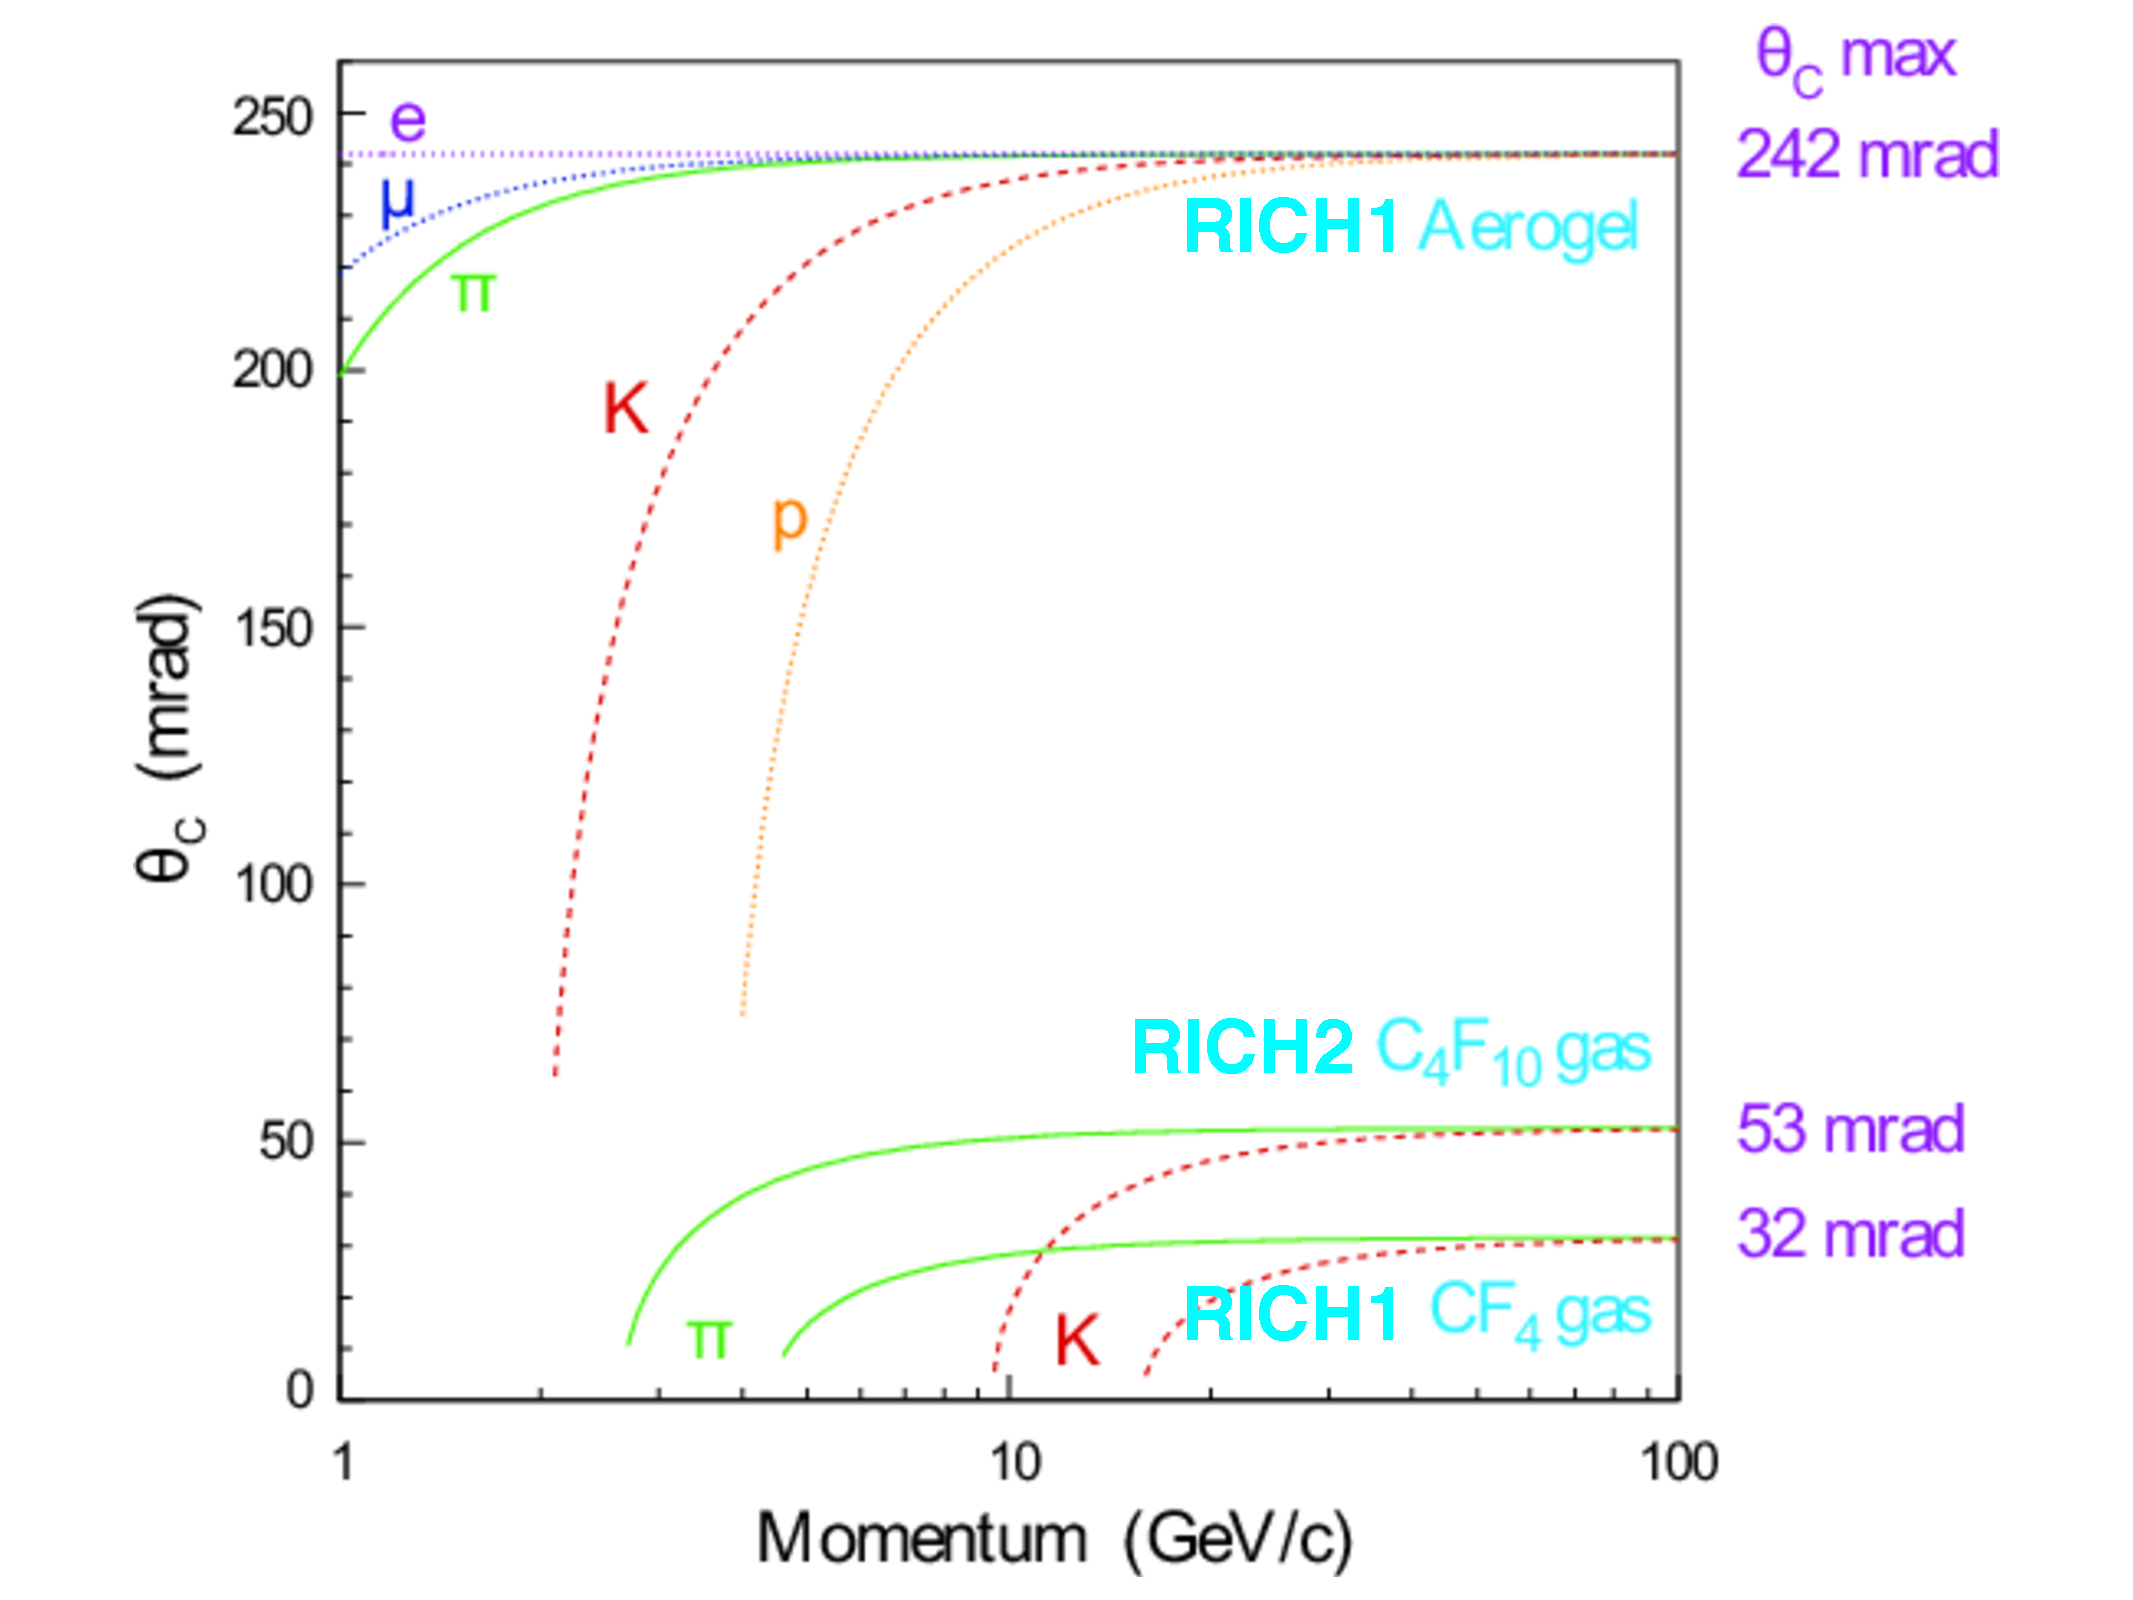
\includegraphics[ width=0.7\textwidth]{./Figs/LHC_LHCb/RICH_radiators.pdf}
  \caption{Expected Cherenkov angles produced by different particles travelling through the different radiators in the RICH detectors~\cite{Alves:2008zz}.}
  \label{fig:RICH_radiator_predictions}
\end{figure}


\begin{figure}[htb]
  \centering
  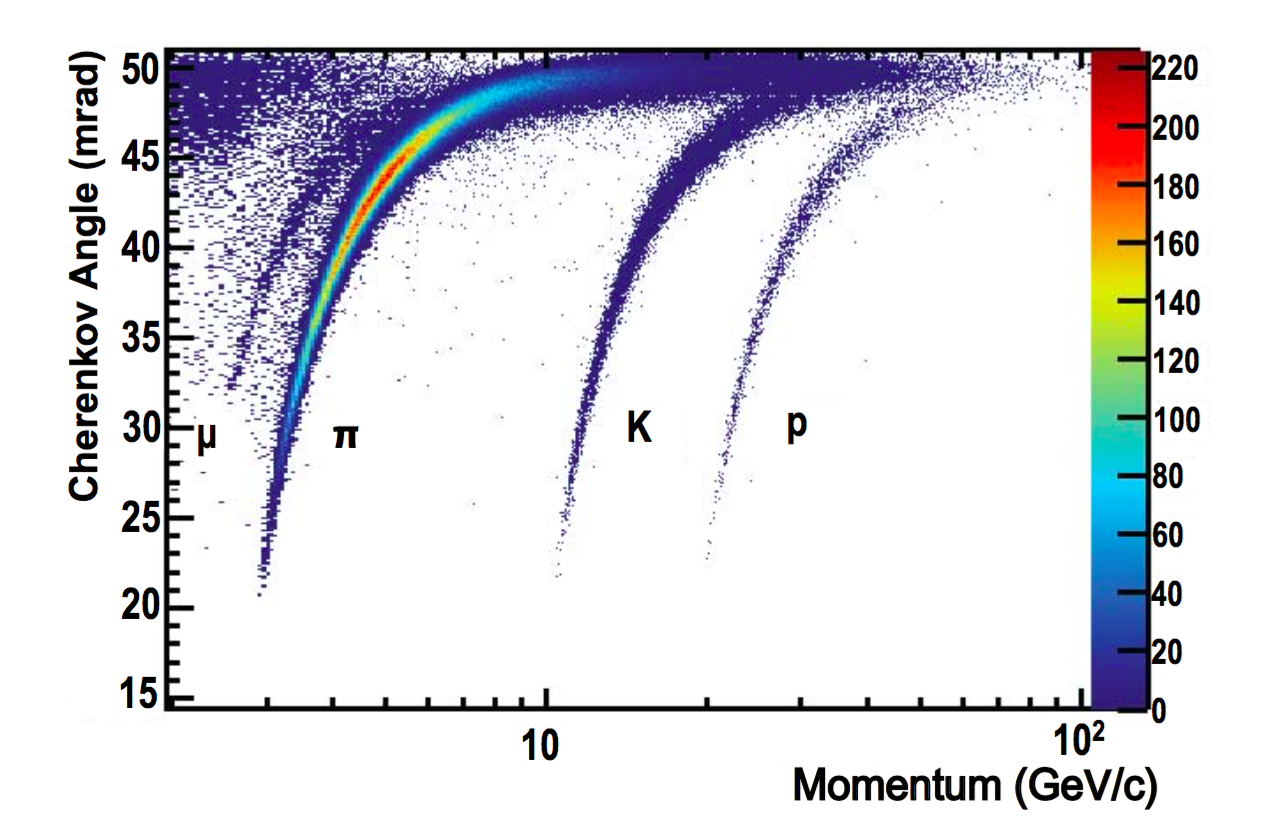
\includegraphics[width=0.8\textwidth]{./Figs/LHC_LHCb/RICH1_performance.png}
  \caption{Cherenkov angles for isolated tracks as a function of momentum in the RICH1 detector for 2011 data \cite{Adinolfi:2012qfa}.}
  \label{fig:RICH_preformance}
\end{figure}


\subsubsection{Calorimeters}
\label{Calo}

The calorimeter system consists of the Scintillating Pad Detector (SDP), Pre-Shower (PS), electromagnetic calorimeter (ECAL) and the hadronic calorimeter (HCAL). The main purposes of the calorimeters are to identify electrons, photons and hadrons with high transverse momentum to be used in the first level of the trigger the L0, and also to help with the reconstruction and identification of these particles. The ECAL is the only part of the LHCb detector that measures the position and energy of photons and neutral pions. 

The calorimeters in LHCb are sampling calorimeters that consist of layers of lead absorbers and scintillating material. In lead, incident particles create showers of secondary particles, the charged particles produced in the absorders create light as they pass through the scintillators. The light travels through wavelength shifters where it is collected by photon multiplier tubes and turned into an electrical signal. In the ECAL showers are started by ionisation, bremsstrahlung radiation or pair production depending on the energy of the incident particle and whether is it a $e^{\pm}$ or a photon. In the HCAL it is interaction via the strong force that leads to showers of secondary particles. The showers produced in the calorimeters are along the direction of flight of the incident particle. Unlike other sub-detectors in LHCb, the calorimeters change the particle as it moves through the detector in order to measure the energy.

The SPD, PS and ECAL identify electrons, positrons and photons. The SPD is a layer of scintillating material at the start of the calorimeter system, it separates electron and photon showers created later in the calorimeter because only charged particles will produce light in the SPD. Next in the calorimeter system is the PS, it consists of a lead absorber followed by another scintillator similar to the SPD, the length of the lead absorber is chosen so that electrons will start showers in the absorber but charged pions will not. There is only a 1$\%$ chance of a pion creating shower in the PS. Information collected by the PS enables showers created by pions in the ECAL to be separated from those created by electrons and positrons. The ECAL is designed to contain the entire shower of high energy photons so that it can provide good energy resolutions of photons passing through the detector. The ECAL has an energy resolution of $\delta E / E = 9\%/\sqrt{(E)} \oplus 0.8\%$  provided information from the PS and SPD are used. 

The HCAL is predominately designed for use in the trigger and there is no requirement that the HCAL contains the full hadronic showers, therefore it was designed with a lower energy resolution of $\delta E / E = 69\% / \sqrt{(E)} \oplus 9\%$. 


\subsubsection{Muon Stations}
\label{Muon_stations}

The muons stations are designed to identify highly penetrating muons, for use in the trigger and offline analyses. Muons are produced in made \bhadron decays, good muon identification is necessary trigger events containing muons and to distinguish topologically similar decays such as \bmumu, \bdkpi, \bskk and \bskpi in physics analyses. 
Compared to other particles muons have a high penetrating power due to their relatively large mass and because muons do not interact via the strong force, these properties are exploited in the muon detectors. 

There are 5 muon stations, M1-5, shown in Figure \ref{fig:muon_system} that track and identify highly penetrating muons. The first muon station is located before the calorimeters, the inner section where the fluence is greatest, is made of gas electron multiplier foils and the outer section is made from multiwire proportional chambers (MWPCs). Stations M2-5 are located after the HCAL, by which point most other particles have been absorbed by the calorimeters. These stations are made from MWPC and between each station is 80cm of lead absorber ensuring only highly penetrating muons pass through the muon detector. A muon must have a momentum of at least 3 GeV/c to pass through the calorimeters and M2 and M3, to travel through all the muons stations a muon must have a momentum of 6~GeV/c. 
The first 3 stations have a high spatial resolution and provide track and transverse momentum information to be used the the trigger. M1 is located before the calorimeters to improve the transverse momentum measurement of the muons. The last two stations have lower spatial resolution and are designed to identify highly penetrating muons. After the muon stations there is an iron wall to stop any particles from travelling downstream of the detector. The size of the muon stations increases with distance from the interaction point to ensure the full angular acceptance of the detector is covered. Tracking information collected in the muon stations can be used in the trigger because the station lie outside the magnetic field which allows for fast reconstruction of the tracks and a muons. 

\begin{figure}[tb]
  \centering
  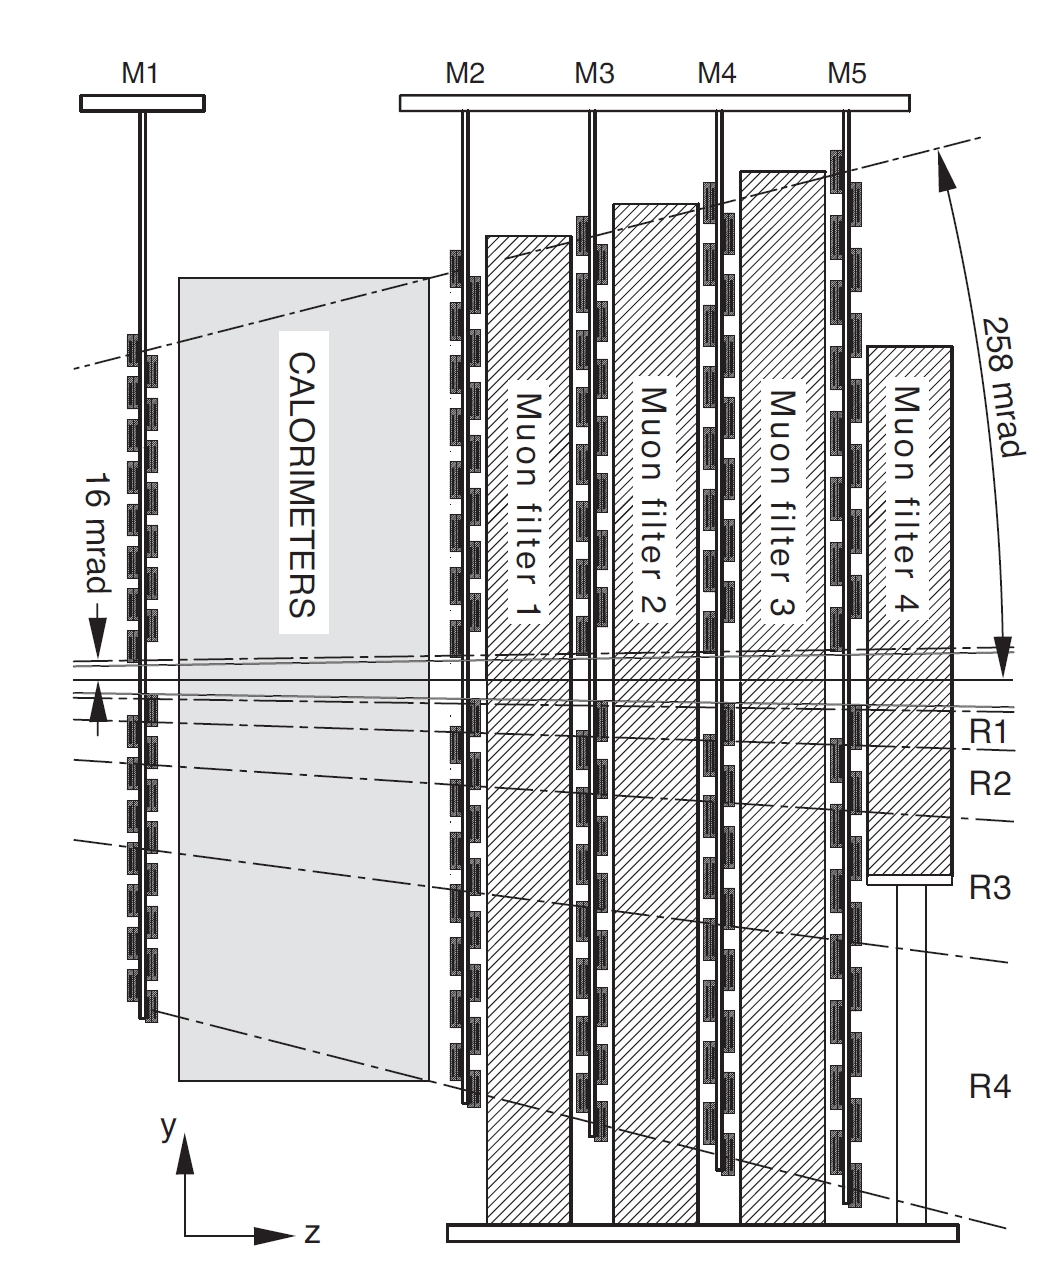
\includegraphics[ width=0.5\textwidth]{./Figs/LHC_LHCb/muon_system.png}
  \caption{Layout of the muon stations~\cite{Alves:2008zz}.}
  \label{fig:muon_system}
\end{figure}

\subsubsection{PID information and performance}
\label{PID_variables}
%There is a plot that shows the usefulness of the RICH PID, this is in Ed Greening's Thesis. 

The information collected in the PID detectors is combined to provide several discriminating variables that can be used to identify muons, protons, kaons, pions and electrons.

The muon stations are used, along with information from the tracking system, to produce a binary selection (isMuon) to identify muons. The tracking system is used to extrapolate a field of interest within the muon stations, a muon is identified if hits in the muon stations can be combined with those from the tracking system within the field of interest. The number of the hits required in the muon stations depends on the momentum of the muon. Muons with momentum in the range 3<$p$<6 GeV must leave hits in M2-3, those in the momentum range 6<$p$<10 muon leave hits in M2-3 and either M4 or M5 and finally muons with momentum above 10 GeV must be observed in all the muon stations. Figure~\ref{fig:isMuon_efficiency} shows the efficiency for the isMuon selection at selecting muons and hadron mis-identification probabilities. The mis-ID rate is higher for lower momentum particles, which is expected given there are less hits in the muons detectors. The main contribution is the misidentifying particles as muons comes from the kaons and pions that decay in flight, the muons from these decays are then detected in the muon stations.


\begin{figure}[htb] 
  \centering    
  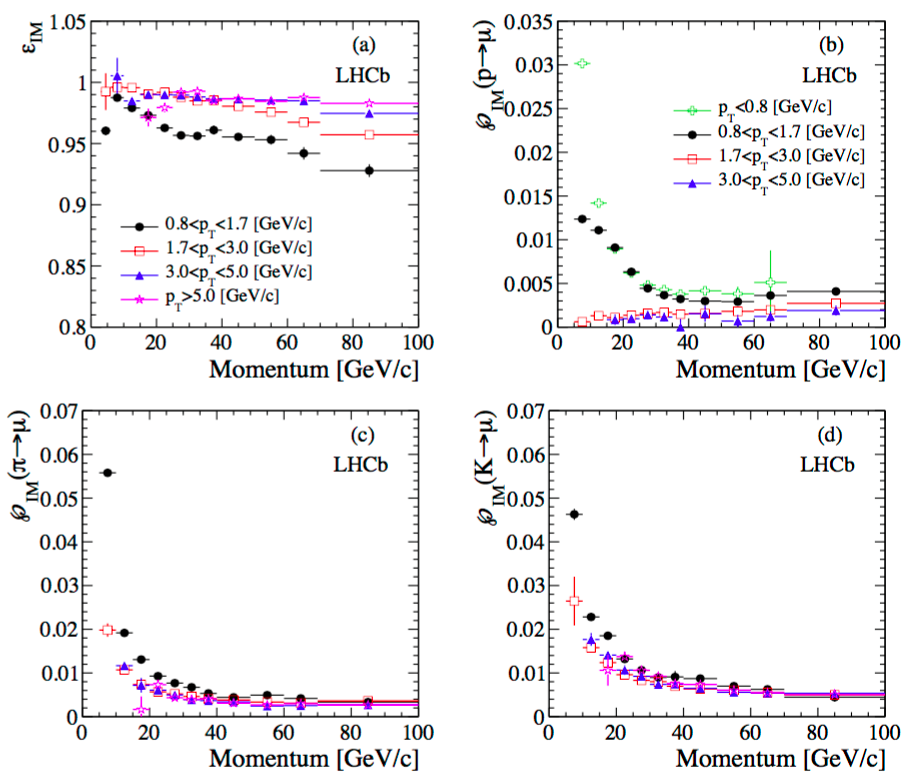
\includegraphics[width=1.0\textwidth]{./Figs/LHC_LHCb/isMuon_eff.png}
  \caption{Muon efficiency (top left) and misidentification probabilities for protons (top right), pions (bottom left) and kaons (bottom right) for isMuon criteria \cite{Archilli:2013npa}.}
  \label{fig:isMuon_efficiency}
\end{figure}




The information from all the PID detectors is combined using two different methods to provide global particle identification variables. One method is based on likelihood fits and the other is based on Neural Networks. In the first method, likelihood fits are performed in each sub-detector comparing each charged particle track to different particle hypotheses. The information from the likelihood fits in each sub detector are combined into a global variable. The final variable is the difference in the log - likelihoods between the track corresponding to a pion and a different particles hypothesis (kaon, proton, muon, electron), it gives a measure of how likely each particle hypothesis is compared to a pion. These variables are known as DLL variables. 




The second method uses information from the PID detectors and the tracking system in Neural Networks to provide a probability of a track having a particular particle hypothesis. This method takes into account correlations between detector systems and extra detector information that are not considered in the likelihood method. The Neural Networks are trained on simulated inclusive $b$ decays and can be tuned to suit different situations, such as the data taking year. The variables produced by the Neural Networks are known as ProbNN variables. 


Figure~\ref{fig:DLL_vs_ProbNN} shows a comparison of the performance of the DLL and ProbNN variables in selecting protons and muons. Although the performance to the two types of variables are quite different, the efficiencies of each variable varies with different kinematic properties of the decay. The most appropriate PID variable type to use depends on the physics analysis it is being used in. 




\begin{figure}[htb] 
  \centering    
  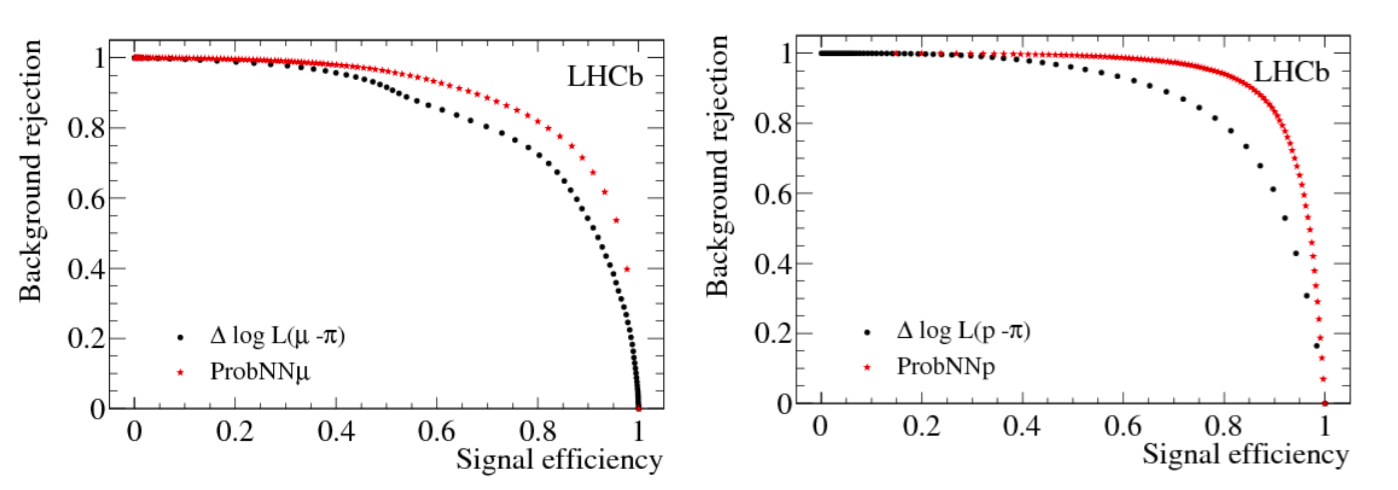
\includegraphics[ width=1.0\textwidth]{./Figs/LHC_LHCb/DLL_vs_ProbNN.png}
  \caption{Muon (left) and proton (right) signal efficiency vs background rejection for DLL and ProbNN PID variables \cite{Alves:2008zz}.}
  \label{fig:DLL_vs_ProbNN}
\end{figure}







\subsection{The Trigger}

\label{Trigger}

The LHC was designed to collide protons at a rate of 40 MHz, this rate is too high for information to be read out of the LHCb detector. However most $pp$ collisions do not produce particles within the detector acceptance that are interesting for physics analyses at LHCb. A trigger system is used that selects potentially interesting events to be saved for later physics analysis. The trigger has been designed to select interesting physics events with a high efficiency  whilst reducing the event rate to one where information from the full detector can be read out.  There are two levels to the LHCb trigger; the hardware trigger and the software trigger. The hardware trigger is know as the level-zero (L0) trigger and reduces the 40~MHz event rate to 1~MHz at which the full detector can be read out. The software trigger is know as the High-Level-Trigger (HLT), it has two stages and runs on the output of the L0 further reducing the event rate by utilising information for all the detector sub-systems. Each level of the trigger is composed of trigger `lines'; these lines are made up of reconstruction and selection algorithms and either accept or reject each event. Only events that are acceptance by a trigger line at both the L0 and HLT are available for use in physics analyses. 

\subsubsection{The L0 trigger}
\label{L0}


The L0 trigger runs synchronously to the LHC bunch crossing. Its purpose is to reduce the events rate to 1~MHz, where information from the full detector can be read out. Therefore the L0 is limited to use information from the detector that can be read at the same rate as the LHC collision rate.
The L0 uses information from 3 parts of the detector, the VELO, calorimeters and the muon stations, to make decisions about the relevance of each event.%; the VELO, calorimeters and the muon stations. 


The pileup veto stations in the VELO are used in L0 pileup trigger lines, these lines identity the number of collisions in an event and are predominatley used for luminosity measurements~\cite{Aaij:2011er}.

The other L0 trigger lines are based on the kinematic properties of \bhadron decays. The heavy masses of \bhadrons means that their decays are characterised by the production of daughter particles with large transverse momentum ($p_{T}$) and transverse energy ($E_{T}$).
%The calorimeters are used to identify events that conating electrons, photons and hadrons with high $E_{T}$. 
The calorimeters are used in trigger lines that select events containing high $E_{T}$ electrons, photons or hadrons. Information from the PS, SPD, ECAL and HCAL is used to identify electrons, photons and hadrons in each event. Events are then accepted by the trigger lines if there is an electron, photon or hadron with $E_{T}$ above a threshold value provided the event multiplicity is not too high. The $E_{T}$ thresholds are different for each particle type. Events with high multiplicity take a long time to reconstruct and process in the HLT, therefore it is not efficiency to keep these events. The multiplicity is measured by the number of hits in the SPD detector (nSPD), only events with nSPD lower than a specified value can pass an L0 trigger line. 


In a similar way to the calorimeters, the muon stations are used to identify muons with high $p_{T}$ for trigger lines. There are two L0 trigger lines for muons that accept events based on muon $p_{T}$ if either a single muon has a $p_{T}$ above a threshold value or if the two muons with this highest $p_{T}$ have $\sqrt{p_{T1} \times p_{T2}}$ above a threshold value, provided the event multiplicity is not too high. %The L0 muon trigger lines are most important to select \bsmumu candidates. The efficiencies for these 2 lines are show in Figure X, most events are triggered by the L0Muon but some are added by the L0Dimuon lines. 

The $E_{T}$ and $p_{T}$ thresholds and the multiplicity limit for the L0 trigger lines vary for each year of data taking depend on the bandwidth available for the trigger. % and are shown in table X. 


\subsubsection{The HLT trigger}
\label{HLT}

Events that are accepted by trigger lines in the L0 are moved to the Event Filter Farm where the HLT is run. The HLT is a software trigger that is split into two levels that are run successively. 


The HLT1 is the first level of the HLT. It runs on the output of the L0 checking the decisions make by the L0 trigger lines and reducing the event rate. % from 1 MHz for processing in the HLT2. 
Time constraints in the HLT1 do not allow for full event reconstruction using all LHCb sub-detectors, instead the HLT1 runs reconstruction and selection algorithms on event information from the VELO and tracking stations. These trigger lines are composed of generic selection criteria, making decisions that confirm those made in the L0 about particular particle types and also identify generic types of particle decays such as inclusive \bhadron decays. The second level of the HLT, HLT2, runs on the output of the HLT1 which provides an event rate that is low enough to allow event reconstruction that includes all detector subsystems. The trigger lines in the HLT2 are designed to select decays relevant to specific physics analyses or particle decay topologies, this is made possible by detailed information from the reconstruction. 

Just like the L0 trigger, trigger lines in the HLT vary for each year of data taking both the selection criteria used in the lines and also new trigger lines are introduced. The number of HLT2 lines increases with each year of data taking as understanding of the capabilities of the experiment increases; there were about 100 HTL2 lines in 2011, 200 in 2012 and 450 in 2015. Furthermore, significant changes were made in the reconstruction used in the HLT between Run 1 and Run 2,  the details of the changes made can be found in \cite{Lupton:2230910}. The majority of the changes to the HLT for Run 2 are not relevant for the analysis discussed in this thesis, the overall impact is that a more detailed reconstruction is used in the decisions of the Run 2 HLT lines compared to Run 1.


\subsubsection{Trigger Decisions}
\label{trigger_decisions}
The trigger lines in the L0 and HLT return three different types of decisions that are used to classify events. The choice of which type of trigger decision to use depends on the particular physics analysis and the signal decay of interest, the decisions can either be used line by line or as global decisions taking all lines together. The different decisions are:
\begin{itemize}
\item {\bf TOS}, `triggered on signal', tracks and hits that make up signal candidate of a physics analysis are sufficient for the event to pass the trigger line. 
\item {\bf TIS}, `triggered independant of signal', if the tracks and hits associated with the signal candidate of a physics analysis are removed from the event, other tracks and hits would still cause the event to pass the trigger line.
\item {\bf Dec}, refers to whether the event was accepted by the trigger line.
\end{itemize}

\subsection{LHCb Software and Simulation}
\label{Software_Simulation}
%Options instead of referenes, Susan references the realease areas!

The data that is read out of the LHCb experiment needs further processing before it can be used in physics analyses. The \textsc{Gaudi} framework~\cite{Mato:1998gfa} is a C++ framework that is the basis for the software applications needed to process the data at LHCb~\cite{Antunes-Nobrega:835156}. This framework ensures that the necessary software is available to all users and changes to the software are implemented across all applications, it is suited to the distributed computing system used in LHCb~\cite{Stagni:2012rs}. 


Once events have been accepted by the trigger, the first step in processing the output of the detector is reconstructing events, this is done by the \textsc{Brunel} application. It takes the digitised detector read out and reconstructs hits in the tracking stations to find particle trajectories and momenta and combines information from the RICH detectors, calorimeters and Muon Stations to compute PID variables. The output of processing by the \textsc{Brunel} application are stored in `Data Summary Type' (DST) files. 

Next the \textsc{DaVinci} application is used to fit the tracks reconstructed in \textsc{Brunel} with primary and secondary vertices. This application assigns particle hypotheses to each track and reconstructs the decay trees of particles in the detector, computing the kinematic properties that are needed for physics analyses. The the reconstructed output of the trigger is too large to be stored in one place and to be used by all the analysts therefore a `stripping' procedure is used to break up the data into a manageable size for physics analyses. Each physics analysis designs a set of loose selection requirements specific to their decay of interest, the selections are applied together to the reconstructed events and are designed to keep as much of the signal as possible but reduce the number background events. Only events that pass a stripping line selection are avaliable to be used in physics analyses. The output of this process are smaller DST files, events passing the stripping selections can either be saved with the full event information or with just the tracks related to the signal candidate. The choice depends on the physics process the stripping line is relevant for. The stripping selection is run a limited number of times and is applied seperately to data collected in different years. Requirements are imposed on the amount of data each stripping line can retain; typically  the output of a line must be less than 0.05~$\%$ of the original data set size if the full event information is saved. Each analyst then uses the DaVinci application one last time to produce \textsc{Root}~\cite{Brun:1997pa} files from the output of their stripping lines, these files display the data in histogram and are used for physics analyses. %RooFit has citation \cite{Verkerke:2003ir}


As well as data collected by the experiment, simulated data that mirrors what is expected in the experiment is needed to understand the detector performance and for physics analyses. There is a set of software applications that are dedicated to the production of Monte Carlo simulated events within the \textsc{Gaudi} framework. Events are generated using the \textsc{Gauss} application~\cite{1742-6596-331-3-032047, Clemencic:2011zza}, this package uses \textsc{Pythia}~\cite{Sjostrand:2006za,Sjostrand:2007gs} to model proton-proton collisions and the production of particles, then the \textsc{Evt}\textsc{Gen}~\cite{Lange:2001uf} application to calculate the decays of these particles. Final state radiation is modelled using \textsc{Photos}~\cite{Golonka:2005pn}. Both \textsc{Pythia} and \textsc{Evt}\textsc{Gen} have been tuned for the production and decay of particles within the LHCb detector. In the simulation the type of particles generated and how they decay can be specified so that the simulated events are relevant to particular physics decays. The detector response to the simulated events is processed by the \textsc{Boole} application with uses \textsc{Geant4}~\cite{Agostinelli:2002hh,Allison:2006ve} to model the detector. The output is a digitised response of the detector which is then processed by \textsc{Brunel} and \textsc{DaVinci} in the same way as the real data to produce \textsc{Root} files that are used in physics analyses. %RooFit has citation \cite{Verkerke:2003ir}

The LHCb software framework is set up so that it can be used on the Worldwide LHC Computing Grid~\cite{Bird:2011zz, WWCG}, the Grid is made up of computers across the world that each store part for the LHCb data set and simulation data. Despite the stripping process the data produced at LHCb is too large to be stored in one place. The \textsc{Dirac}~\cite{Paterson:1397926} system manages grid sites and the \textsc{Ganga} project allows the submission analysis code to different grid sites. The grid enables analysts to process and study the large amounts of data produced by LHCb without having to store the data where the analyst is. 





\subsection{LHCb data collected so far}
\label{LHCb_data}
%Need to find some references for the future projections I suppose. 
The data taking periods of the LHC can be split up into different `Runs' which are separated by Long Shut Down periods when maintenance and upgrades are performed on the LHC, the detectors and the accelerator chain that delivers protons to the LHC. Run 1 began in 2010 and ended in 2013, during this Run the LHC operated at two different centre-of-mass energies. In 2010 and 2011 the LHC delivered proton collisions a a centre-of-mass energy of 7~\tev, this was increased to 8~\tev in 2012. The luminosity recored by LHCb in each was; 0.04~\fb in 2010, 1.10~\fb in 2011 and 2.08~\fb in 2012. After Run~1 the LHC and experiment entered the Long Shutdown~1 (LS1) when the machine and experiments were prepared to deliver and detect proton collisions at $\sqrt{s}$~=~13. Run~2 began in early 2015 and is still on going, so far LHCb has recorded 0.32~\fb in 2015 and 1.67~\fb in 2016 both at a centre-of-mass energy of 13 TeV. Figure~\ref{fig:LHCb_lumi} shows the integrated luminosity collected by LHCb in each year of data taking. The recorded luminosity of Run~2 is currently less that what was recorded in Run~1, however the production cross section for \bhadrons approximately doubled with the increase in centre-of-mass energy between Run~1 and Run~2 therefore the Run~2 data set will already contain more \bhadrons useful for physics analyses than the Run 1 data set. 


The expected end of Run~2 is 2018 by which time LHCb is expected to have recorded 5~\fb luminosity during the Run. Run~2 will be followed by a second long shut down period (LS2) in which LHCb shall be upgraded ready to record proton collisions at 14~\tev during Run~3. This run of data taking is expected to be from 2021 - 2024 and by the end of Run~3 LHCb is expected to have collected an integrated luminosity of 23~\fb over all the runs. 

The physics analysis described in this thesis uses the full data sets from Run~1 and 2015 and data taken up to September during 2016. The 2016 data set is therefore reduced to 1.1~\fb.

\begin{figure}[htb] 
  \centering    
  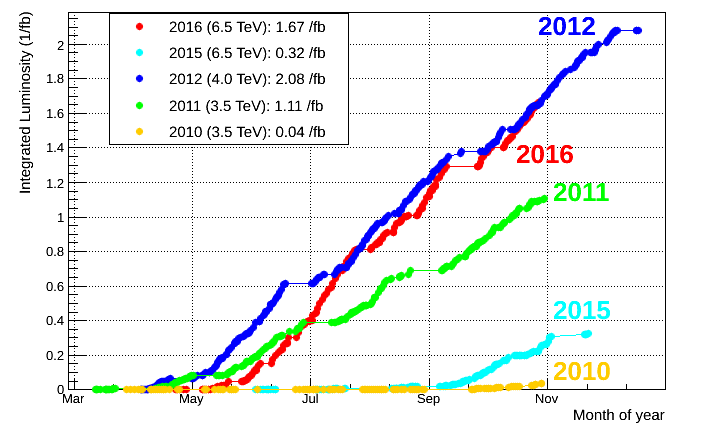
\includegraphics[ width=0.8\textwidth]{./Figs/LHC_LHCb/IntLumiRun1-2.png}
  \caption{Integrated luminosity collected by the LHCb experiment in each year of data taking. Source: LHCb.}
  \label{fig:LHCb_lumi}
\end{figure}


%\begin{figure}[htb] 
%  \centering    
%  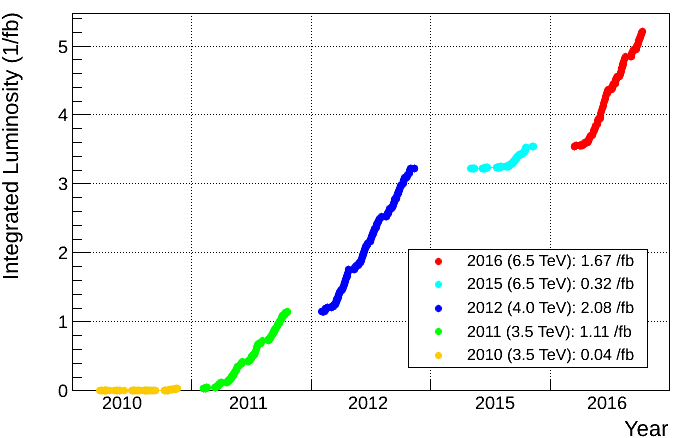
\includegraphics[ width=0.8\textwidth]{./Figs/LHC_LHCb/IntegratedLumiCumul.png}
%  \caption{Cumulative integrated luminosity collected over data taking years at the LHCb experiment. Source: LHCb.}
%  \label{fig:LHCb_lumi_cuml}
%\end{figure}


